\documentclass[preprint,authoryear,a4paper,10pt,onecolumn]{elsarticle}
\usepackage[british,english]{babel}
\usepackage{mathpazo}
\usepackage[T1]{fontenc}
\usepackage[latin9]{inputenc}
\usepackage{float}
\usepackage{amsmath}
\usepackage{graphics}
\usepackage{setspace}
\usepackage{amssymb}
\usepackage{natbib}
\usepackage[title]{appendix}
\usepackage{siunitx}

\makeatletter
\newfloat{algorithm}{H}{loa}[section]
\floatname{algorithm}{Algorithm}
%\newcounter{algorithm}
\journal{Neuroimage}
\def\argmin{\mathop{\operator@font arg\,min}} 
\def\argmax{\mathop{\operator@font arg\,max}} 
\makeatother

\begin{document}

\begin{frontmatter}

\title{QuickBundles for Effective Real-Time Tractography Clustering}

\author[UC]{Eleftherios Garyfallidis}
\ead{garyfallidis@gmail.com}
\address[UC]{University of Cambridge, Wolfson College, Barton Road, Cambridge CB3 9BB, UK}

\author[Berkeley]{Matthew Brett}
\ead{matthew.brett@gmail.com}
\address[Berkeley]{University of California, Henry H. Wheeler, Jr. Brain Imaging Center, 10 Giannini Hall, Berkeley, CA 94720,USA}

\author[CBU]{Marta Correia} 
\ead{marta.correia@mrc-cbu.cam.ac.uk}
\address[CBU]{MRC Cognition and Brain Sciences Unit, 15 Chaucer Road, Cambridge CB2 7EF, UK}

\author[WBIC]{Guy Williams} 
\ead{gbw1000@wbic.cam.ac.uk}
\address[WBIC]{The Wolfson Brain Imaging Centre, University of Cambridge, Box 65, Addenbrooke's Hospital, Cambridge CB2 0QQ, UK}

\author[CBU]{Ian Nimmo-Smith\corref{Cor}} 
\ead{iannimmosmith@gmail.com}
\cortext[Cor]{Corresponding author -- Fax +44 (0) 1223 359 062}

\begin{abstract}
  Diffusion MR white matter tractography algorithms generate datasets
  (tractographies) with a very large number of tracks. Their size makes
  it difficult to interpret, visualize and interact with
  tractographies. This is even more of an issue when several
  tractographies are being considered together. To overcome this
  drawback, we present a clustering algorithm, QuickBundles (QB), that
  simplifies the complexity of these large datasets and provides
  anatomically meaningful clusters in seconds with minimum memory
  consumption. Each QB cluster can be represented by a single track,
  which collectively can be visualised as a first sketch of the
  tractography.  Representative tracks from this QB sketch can be
  selected and the associated tracks re-clustered in turn via QB. This
  allows one to explore the neuroanatomy directly. Alternatively the QB
  sketch can be used as a precursor tractography of reduced
  dimensionality for input to other algorithms of higher order
  complexity, resulting in their greater efficiency. Beyond these
  fundamental uses we show how QB can help identify hidden structures,
  find landmarks, create atlases, and compare and register
  tractographies.
\end{abstract}

\begin{keyword}
Tractography;
Diffusion MRI;
Fiber clustering;
White matter atlas;
Direct tractography registration;
Clustering algorithms;
DTI
\end{keyword}
\end{frontmatter}

\section{Introduction}

Following the acquisition of diffusion MR scans, processes of
reconstruction and integration (track propagation) are performed to
create a tractography: a data set composed of tracks, which are
sequences of points in 3D space. Irrespective of the types of
reconstruction and integration a tractography can contain a very large
number of tracks (up to $10^6$) depending principally on the number of
seed points used to generate the tractography but also on how the
propagation algorithm handles voxels with underlying fiber crossings.

The size of these tractographies makes them difficult to interpret and
visualize. A clustering of some kind seems to be an obvious route to
simplify the complexity of these data sets and provide a useful
segmentation.  As a result, during the last 10 years there have been
numerous efforts by many researchers to address both unsupervised and
supervised learning problems of brain tractography. Though these studies
do provide many useful ideas, all these methods suffer ultimately from
lack of practical efficiency.

Current clustering techniques and the principal studies that have applied them to tractographies include:
\textit{Hierarchical clustering} \citep{Visser2010,
  gerig2004analysis, Guevara2010, zhang2005dti, jianu2009exploring};
\textit{$k$-means} \citep{ElKouby2005, Tsai2007}; \textit{Adaptive mean
  shift} \citep{zvitia2008adaptive, Zvitia2010}; \textit{Graph theoretic
  segmentation} \citep{brun2004clustering}; \textit{$k$-nearest
  neighbours} \citep{Ding2003a}; \textit{Generalized Procrustes Analysis
  and Principal Components Analysis (PCA)} \citep{Corouge2004,
  corouge2004towards, Corouge2006}; \textit{Spectral embedding}
\citep{ODonnell_IEEETMI07}; \textit{EM clustering}
\citep{Maddah_MICCA2005, maddah2006statistical, Maddah_IEEEBI2008,
  ziyan2009consistency}; \textit{Spectral clustering}
\citep{jonasson2005fiber}; \textit{Affinity propagation}
\citep{leemans17new, malcolm2009filtered}; \textit{Hierarchical
  Dirichlet process mixture model} \citep{wang2010tractography};
\textit{Current models} \citep{Durrleman2009,
  durrleman2010registration}.

Most of these proposed tractography clustering algorithms are very slow and many
need to calculate a matrix of inter-track distances of size $\mathcal{O}(N^2)$.
This number of computations puts a very heavy load on clustering algorithms,
making them hard to use for everyday analysis as it is difficult to compute all
these distances or store them in memory. For the same reason, no current
algorithm is practical for real time clustering on a large number of tracks. The
heavy computational demands of clustering adds a further overhead to the use of
tractography for clinical applications but also puts a barrier on understanding
and interpreting the quality of diffusion data sets.

To address these key issues of time and space we present a stable,
generally linear time clustering algorithm that can generate meaningful
clusters of tracks in seconds with minimum memory consumption. In our
approach we do not need to calculate all pairwise distances unlike most
of the other existing methods. Furthermore we can update our clustering
online or in parallel. In this way we can overcome the previous barriers
of space and time.

We show that we can generate these clusters \textasciitilde1000 times faster than
any other available method before even applying further
acceleration through parallel processing, and that it can be used to
cluster from a few hundred to many millions of tracks.

Moreover our new algorithm leads to many valuable additional results. QB
can either be used on its own to explore the neuroanatomy directly, or
it can be used as a precursor tool which reduces the dimensionality of
the data, which can then be used as an input to other algorithms of
higher order complexity, resulting in their greater efficiency. Beyond
the use of this algorithm to simplify tractographies, we show how it can
help identify hidden structures, find landmarks, create atlases, and
compare and register tractographies.

\section{Methods}

\subsection{The QB algorithm\label{sub:QB-description}}

QuickBundles (QB) is a very fast algorithm which can simplify
tractography representation to a simple structure in a time that is
linear in the number of tracks $N$; it is an extended update on our
preliminary work~\citep{EGMB10}.

In QB each item, a track, is a fixed-length ordered sequence of points
in $\mathbb{R}^{3}$, and QB uses metrics and amalgamations which take
account of and preserve this structure.  Moreover each item is either
added to an existing cluster on the basis of a distance between the
cluster descriptor of the item and the descriptors of the current set of
clusters. Clusters are held in a list which is extended according to
need. Unlike amalgamation clustering algorithms such as
$k$-means~\citep{steinhaus1956division, macqueen1967some} or
BIRCH~\citep{zhang1997birch}, there is no reassignment or updating phase
-- once an item is assigned to a cluster it stays there, and clusters
are not amalgamated. 

A track is a ordered sequence of points in $\mathbb{R}^{3}$.  The clustering
algorithm needs a measure of distance between two tracks, and QB uses a
particular distance measure that we call minimum average direct flip (MDF).  The
MDF measure requires that each track be resampled to have $K$ points. We
describe the MDF measure and the resampling in
section~\ref{sub:track-distances}.

We index the tracks with $i = 1 \dots N$ where $\mathbf{s}_{i}$ is the
$K\times3$ matrix representing track $i$.

QB stores information about clusters in \emph{cluster nodes}.  The cluster node
is defined as $c=(I,\mathbf{h},n)$ where $I$ is the list of the integer
indices $i = 1 \dots N$ of the tracks in that cluster, $n$ is the number of
tracks in the cluster, and $h$ is the \emph{track sum}. $\mathbf{h}$ is a $K
\times3$ matrix which can be updated online when a track is added to a cluster
and is equal to:
\begin{equation}
  \mathbf{h}=\sum_{i=1}^{n}\mathbf{s}_{i}
\end{equation} 
where $\mathbf{s}_{i}$ is the $K\times3$ matrix representing track $i$,
$\Sigma$ here represents matrix addition, and $n$ is the number of
tracks in the cluster. One summary of the cluster node is the centroid or
\emph{virtual} track $v$ where:

\begin{equation}
  v = \mathbf{h} / n
\end{equation}

The algorithm proceeds as follows.  At any one step in the algorithm we
have $|C|$ cluster nodes. Select the first track $s_{1}$ and place it in
the first cluster node $c_{1}\leftarrow(\{1\},s_{1},1)$.  Obviously $|C|
= 1$ at this point.  For each remaining track in turn $i = 2 \dots N$: (i)
calculate the MDF distance between track $s_{i}$ and the virtual tracks
$v_{e}$ of all the current clusters $c_{e}$, $e = 1 \dots |C|$, where
$v$ is defined on the fly as $\mathbf{v}=\mathbf{h}/n$; (iii) if any of
the MDF values $m_{e}$ are smaller than a distance threshold $\theta$,
add track $i$ to the cluster $e$ with the minimum value for $m_{e}$;
$c_{e}=(I,\mathbf{h},n)$, and update
$c_{e}\leftarrow(I\cup\{i\},\mathbf{h}+s,n+1)$; otherwise create a new
cluster $c_{|C|+1}\leftarrow(\{i\},s_{i},1)$, $|C|\leftarrow|C|+1$.

Popular amalgamation clustering algorithms such as
$k$-means~\citep{steinhaus1956division, macqueen1967some} require
iterative reassignment of items to different clusters and hence do not
run in linear time. Others such as BIRCH~\citep{zhang1997birch} have
linear time performance while imposing limits on the size and spread of
clusters; BIRCH clusters may be contiguous and the BIRCH algorithm
requires further phases of cluster amalgamation to optimise search time
when adding future items. By contrast when QB assigns an item to a node
it stays there, and clusters are not amalgamated.  For further
discussion of the relationship between QB and BIRCH see
section~\ref{sub:BIRCH}.

Choice of orientation can become an issue when using the MDF distance
and adding tracks together, because the diffusion signal is symmetric
around the origin, and therefore the $K \times 3$ track can equivalently
have its points ordered $1 \dots K$ or be flipped with order $K \dots
1$; the diffusion signal does not allow us to distinguish betweeen these
two directions. A step in QB takes account of the possibility of needing
to perform a flip of a track before adding it to a representative track
according to which direction produced the MDF value.

The complete QB algorithm is described in formal detail in
Alg.~\ref{Alg:QuickBundles} and a simple step by step visual example is given in
Fig.~\ref{Fig:LSC_simple}.  One of the reasons why QB has on average linear time
complexity derives from the structure of the cluster node: we only save the sum
of current tracks $h$ in the cluster and the sum is cumulative; moreover there
is no recalculation of clusters, the tracks are passed through only once and a
track is assigned to one cluster only.  There is more detail about this and other in
section~\ref{sub:BIRCH}.

\begin{figure}
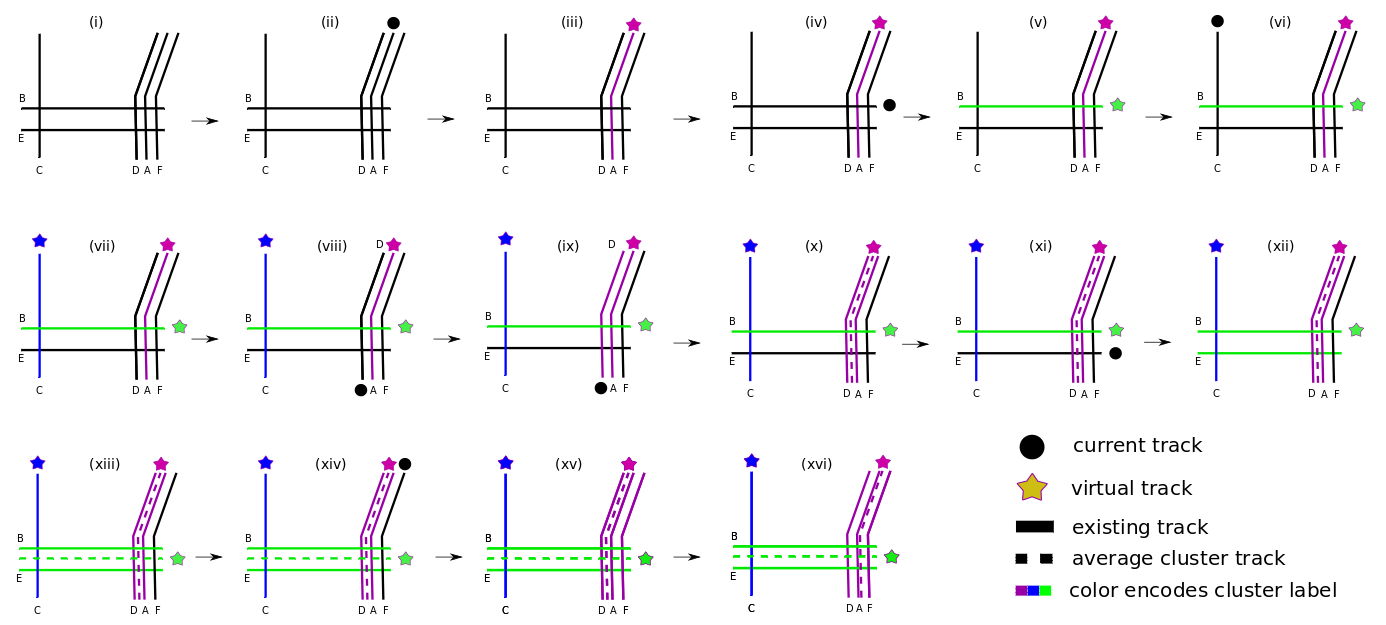
\includegraphics[scale=0.25]{Fig_1_QB_algorithm}
\caption{QB step-by-step: Initially in panel (i) 6 unclustered tracks
  (A-F) are presented; imagine that the distance threshold $\theta$ used here is
  the same as the MDF distance (Eq.~\ref{eq:direct_flip_distance}) between B and
  E: $\theta = MDF(B,E)$. The algorithm starts and in (ii) we see that track A
  was selected; as no other clusters exist track A becomes the first cluster
  (labelled with purple color) and the virtual track of that cluster is
  identical with A as seen in (iii); next in (iv) track B is selected and we
  calculate the MDF distance between B and the virtual track of the other
  clusters. For the moment there is only one cluster to compare so QB calculates
  MDF (B,virtual-purple) and this is obviously bigger than threshold $\theta$
  ($\theta = MDF(B,E)$).  Therefore a new cluster is assigned for B, and B
  becomes the virtual track of that cluster as shown in (v). In (vi) the next
  track C is selected and this is again far away from both purple and blue
  virtuals; therefore another cluster is created and C is the virtual of the
  blue cluster as shown in (vii).  In (viii) track D is selected and after we
  have calculated MDF(D,purple), MDF(D,Blue) and MDF(D,green) it is obvious that
  D belongs to the purple cluster as MDF(D,purple) is smaller and lower than
  threshold as shown in (ix).  However we can now see in (x) that things change
  for the purple cluster because the virtual track is not anymore made by only
  one track but it is the average of D and A shown with a dashed line. In (xi) E
  is the current track and will be assigned to the green cluster as shown in
  (xii) because MDF(E,virtual green) = MDF(E,B) = $\theta$, and in (xiii) we see
  the updated virtual track for the green cluster which is equal to (B+E)/2
  where + means track addition. In (xiv) the last track is picked and compared
  with the virtual tracks of the other 3 clusters; obviously MDF(F,purple) is
  the only distance smaller than threshold, and so F is assigned to the purple
  cluster in (xv).  Finally, in (xvi) the virtual purple track is updated as
  (D+A+F)/3. As there are no more tracks to select, the algorithm stops. We can
  see that all three clusters have been found and all tracks have been assigned
  successfully to a cluster.
  \label{Fig:LSC_simple}}
\end{figure}

\subsection{\label{sub:track-distances}Track distances and preprocessing}

A wide range of approaches have been taken in the literature for
representing or coding for tractographies. The approach we have taken with track
coding has gone in parallel with the selection of appropriate metrics for
inter-track distances.  Numerous inter-track distance metrics have been
proposed~\citep{Ding2003, MaddahIPMI2007, zhang2005dti}. The most common is the
Hausdorff distance~\citep[and many other
studies]{corouge2004towards}. There are two primary disadvantages of
this metric: (1) it ignores the sequential nature of the tracks and
treats each track simply as a cloud of points, and (2) its computation
requires every point on the first track to be compared with every point
on the second track, and vice versa. For these reasons we have opted to
use a very simple symmetric distance \citep{EGMB10, Visser2010} which we
call Minimum average Direct-Flip (MDF) distance $MDF(s,s')$ between
track $s$ and track $s'$, see Eq.~(\ref{eq:direct_flip_distance}). This
distance can be applied only when both tracks have the same number of
points. Therefore we assume that an initial downscaling of tracks has
been implemented, where all segments on a track have approximately the
same length, and all tracks have the same number of points $K$, and segments
$K-1$, which are much less than the number of points or segments in the typical
raw track.  Under this assumption MDF is defined as:

\begin{eqnarray}
\textrm{MDF}(s,s') & = & \min(d_{\textrm{direct}}(s,s'),d_{\textrm{flipped}}(s,s')),\,\,\textrm{where}\label{eq:direct_flip_distance}\\
d_{\textrm{direct}}(s,s') & = & \frac{1}{K}\sum_{i=1}^{K}|x_{i}-x_{i}'|,\,\,\textrm{and}\nonumber\\
d_{\textrm{flipped}}(s,s') & = & \frac{1}{K}\sum_{i=1}^{K}|x_{i}-x_{K-i}'|.\nonumber
\end{eqnarray}
\noindent
Here $K$ is the number of points $x_{i}$ and $x_{i}'$ on the two tracks $s$ and $s'$
and $|x-x'|$ denotes the euclidean distance between two points $x$ and
$x'$.

\begin{figure}
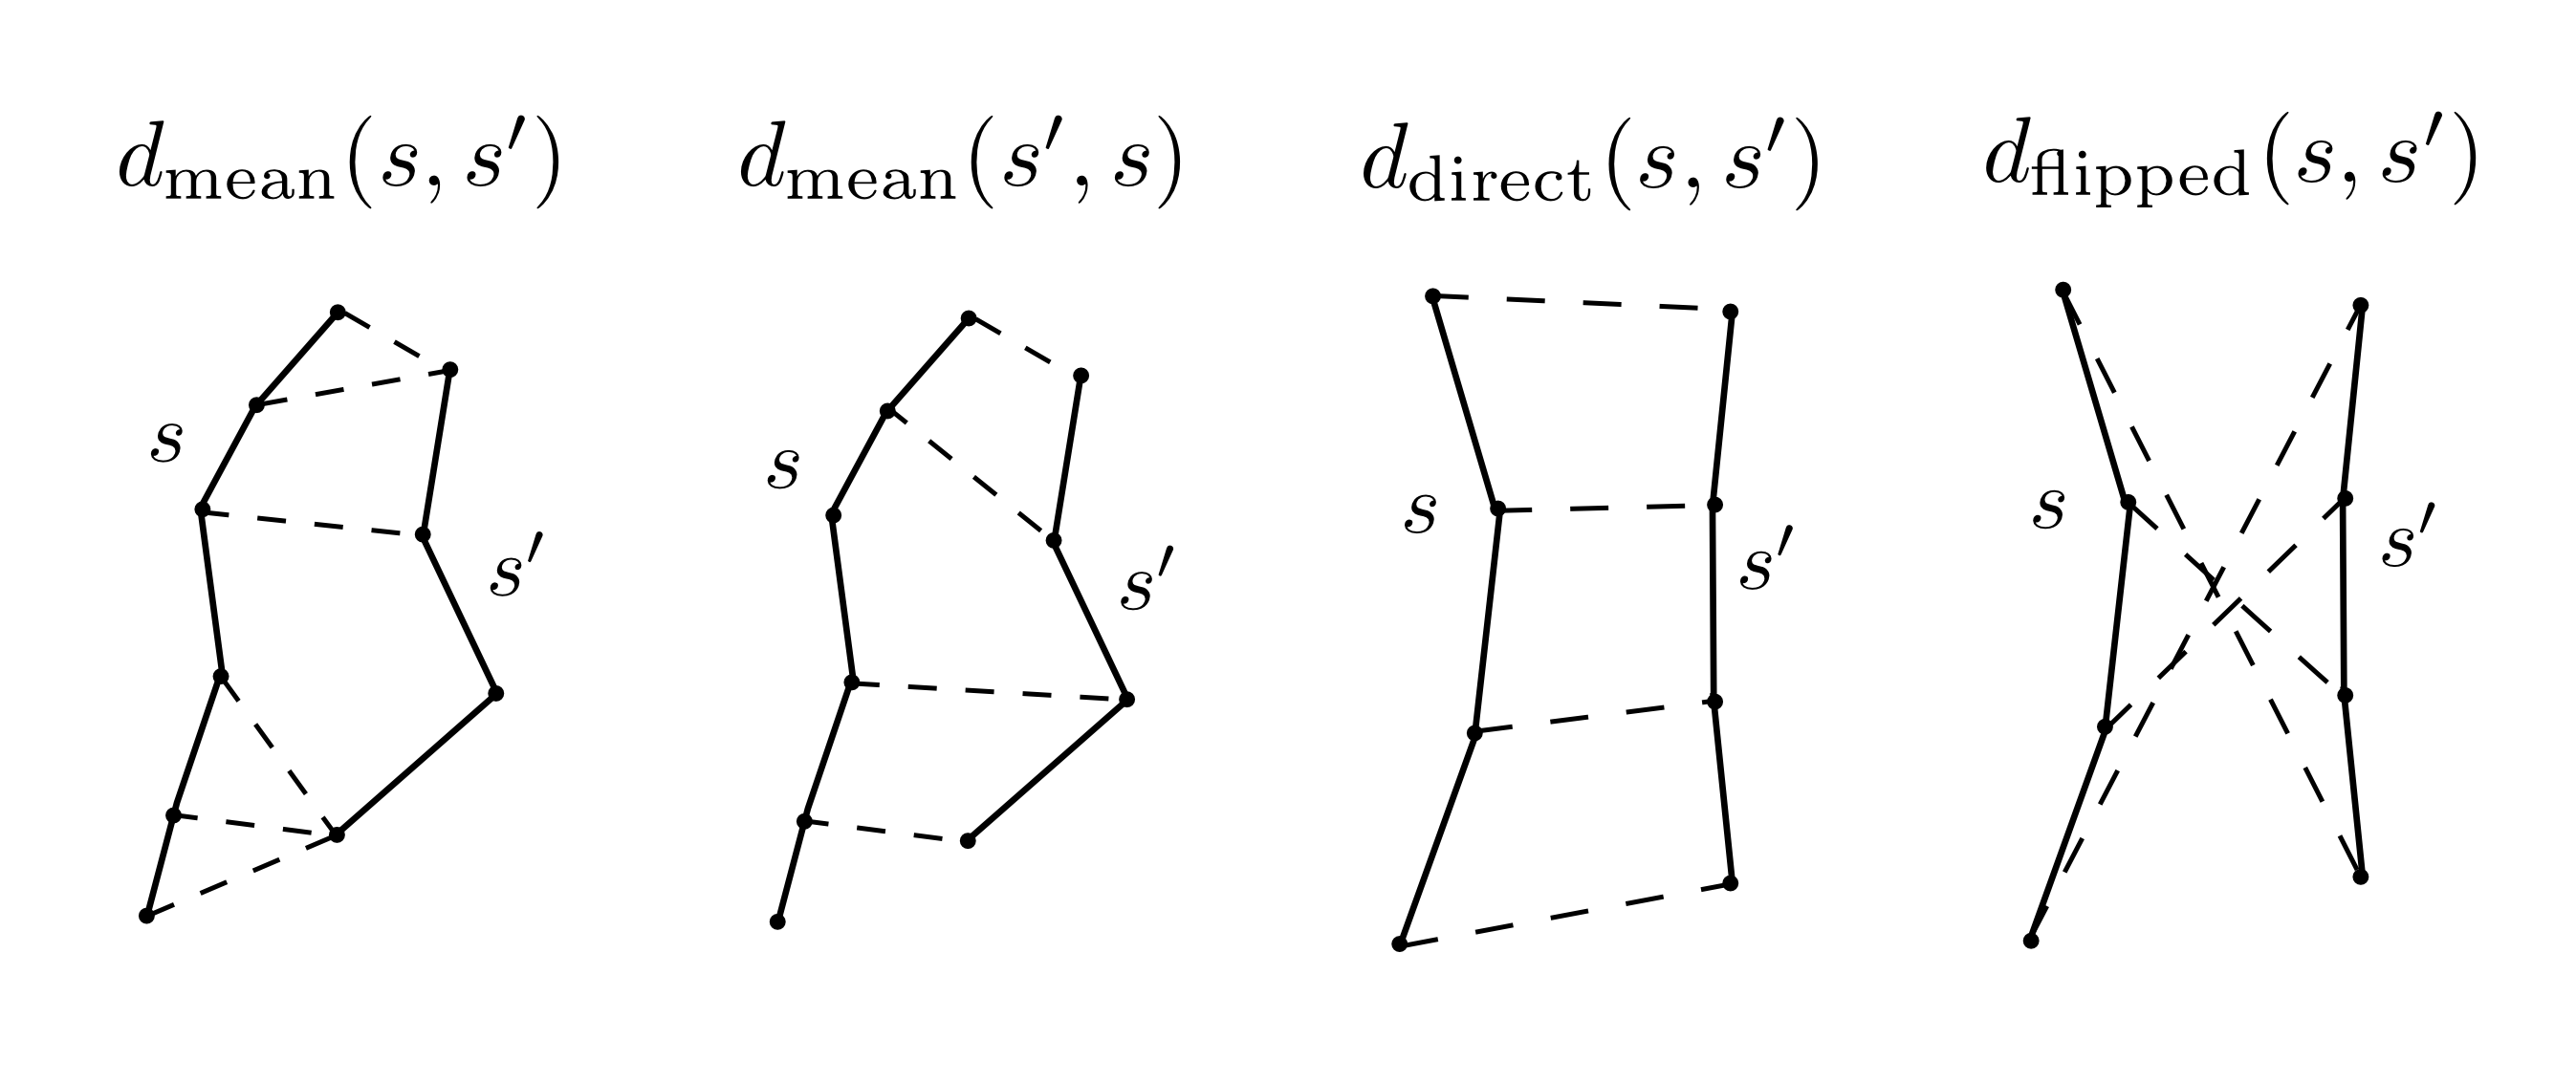
\includegraphics[scale=0.5]{Fig_2_distances2}
\centering{}
\caption{The principal distance used in this work is minimum average direct flip
distance $\textrm{MDF}=\min(d_{\textrm{direct}},d_{\textrm{flipped}})$ which is
a symmetric distance that can deal with the track bi-directionality problem; it
works on tracks which have the same number of points.  Another distance is the
mean average distance which is again symmetric but does not require the tracks
to have the same number of points
$\textrm{MAM}_{\textrm{mean}}=(d_{mean}(s,s')+d_{mean}(s',s))/2$ (see Eq.
(\ref{eq:mean_average_distance})).  In this figure the components of both
distances are shown; the tracks are drawn with solid lines, and then with dashed
lines we connect the pairs of points of the two tracks whose distances
contribute to the overall metric. Note that we cannot calculate the
$\textrm{MDF}$ between the tracks on the left of the figure because they have
different numbers of points.
\label{Flo:Distances_used}}
\end{figure}

The main advantages of the MDF distance are that it is fast to compute,
it takes account of track direction issues through consideration of both
direct and flipped tracks, and that it is easy to understand how it
behaves, from the simplest case of parallel equi-length tracks to the
most complicated with very divergent tracks. Another advantage is that
it separates short tracks from long tracks; a track A that is half the length of
track B will be relatively poorly matched on MDF to B.  

Another important advantage of having tracks with the same number of points is
that we can easily do pairwise calculations on them; for example add two or more
tracks together to create a new average track. We saw in the previous section
how track addition is a key property that we exploit in the QB clustering
algorithm.

Care needs to be given to choosing the number of points required in a
track (track downsampling). We always keep the endpoints intact and then
downsample in equidistant segments. One consequence of short tracks
having the same number of points as long tracks is that more of the
curvature information from the long tracks is lost relative to the short
tracks i.e. the short tracks will have higher resolution.  We found
empirically that this is not an important issue and that for clustering
purposes even downsampling to only $K=3$ points in total can be useful
\citep{EGMB10}. Depending on the application, more or fewer points can
be used. In the results presented in this paper we use $K=12$ except
in~(\ref{sub:Complexity}).


\subsection{Exemplar tracks\label{sub:exemplars}}

The virtual tracks created by QB have very nice properties as they
represent an average track which can stand as the most characteristic
feature of the cluster that they belong to. However, now that we have
segmented our tractography into small bundles, we can calculate many more
potentially important descriptors for the cluster. One of the most
useful approaches is the calculation of exemplars.

Here the idea is to identify an actual track belonging to the
tractography which corresponds in some way to the virtual track. In
other words to find an exemplar or centroid track. Virtual tracks do not
necessarily coincide with real tracks as they are just the outcome of
large amalgamations. There are many strategies for how to select good
exemplars for the bundles. A very fast procedure that we use in our
work is to find which real track from the cluster is closest (by MDF
distance) to the virtual track. We will call this exemplar track $e_{1}$,
i.e.~$e_{1}={\displaystyle \argmin_{x\in C}}\textrm{\,\ MDF}(v,x)$.
The computational complexity of finding $e_{1}$ is still linear in
cluster size, and that will be very useful if we have created
clusterings with clusters containing more than \textasciitilde5000 tracks
(depending on system memory).

A different exemplar can be defined as the most typical track among all
tracks in the bundle, which we denote by $e_{2}={\displaystyle
  \argmin_{x\in C}}\,{\displaystyle \sum_{y\in C}}\mathrm{MDF}(y,x)$, or
if we want to work with tracks with possibly different numbers of points
we could instead use $e_{3}={\displaystyle \argmin_{x\in
    C}}\,{\displaystyle \sum_{y\in C}}\mathrm{MAM}(y,x)$.
Identification of exemplar tracks of type $e_{2}$ and $e_{3}$ will be
efficient only for small bundles of less than $5000$ tracks because we
need to calculate all pairwise distances in the bundle. We show below
many applications of the exemplars. 

In summary, a virtual (centroid) track is the average of all tracks in
the cluster. We call it virtual because it does not really exist in the
real data set, and to distinguish it from exemplar (medoid) tracks which
are again descriptors of the cluster but are represented by real tracks.

\subsection{Tightness Comparisons\label{sub:Tightness-comparisons-1}}

We have found rather few systematic ways to compare different clustering
results for tractographies in the literature
\citep{moberts2005evaluation}.  Being able to compare results of
clusterings is crucial for creating stable brain imaging procedures, and
therefore it is necessary to develop a way to compare different
clusterings of the same subject or different subjects. Although we
recognise that this is a difficult problem, we propose the following
approach with a metric which we call tight comparison (TC). Tight
comparison works as follows. Let us assume that we have gathered the
exemplar tracks from clustering A in $E_{A}=\{e_{1},...,e_{|E_{A}|}\}$
and from clustering B in $E_{B}=\{e_{1}^{'},...,e_{|E_{B}|}^{'}\}$ where
$|E|$ denotes the number of exemplar tracks of each clustering $E$. The
size of set $E_{A}$ does not need to be the same as that of
$E_{B}$. Next, we calculate all pairwise MDF distances between the two
sets and store them in rectangular matrix $D_{AB}$. The mimima of the
rows of $D_{AB}$ provide the distance to the nearest track in B of each
track in A ($E_{A\rightarrow B}$) and similarly the minima of the
columns of $D_{AB}$ the distance to the nearest track in $A$ of each
track in B ($E_{B\rightarrow A}$). From these correspondences we only
keep those distances that are smaller than a tight (small) threshold
$\theta$. Then we define TC (Tightness Comparison) to be

\begin{equation}
TC=\frac{1}{2}\left(\frac{|E_{A\rightarrow B}\leq \theta |}{|E_{A}|}+\frac{|E_{B\rightarrow A}\leq \theta |}{|E_{B}|}\right)\label{eq:TC}
\end{equation}

\noindent where $|E_{A\rightarrow B}\leq \theta |$ denotes the number of
exemplars from A which had a neighbour in B that is closer than $\theta$
and similarly for $|E_{B\rightarrow A}\leq \theta |$ the number of
exemplars from B to A which their distance was smaller than
$\theta$. In other words, $TC$ is mean of the fraction of row minima of
$D_{AB}$ that are less than $\theta$ and the fraction of column minima
less than $\theta$.  When $TC=0$ that means that every exemplar from the
one set was further than $\theta$ to all exemplars in the other
set. When $TC=1$ then all exemplars from one set had a close neighbour
in the other set. This metric is extremely useful especially when
comparing tractographies from different subjects because it does not
require $|E_{A}|=|E_{B}|$.

\subsection{Merging two sets of bundles\label{sub:merging}}

We can merge bundles using exemplar tracks or virtual tracks. We first
set a distance threshold $\theta$ usually the same as the one we used
for the QBs in the previous step. Assume now that we have gathered the
virtual tracks from clustering A in $V_{A}=\{v_{0},...,v_{|V_{A}|}\}$
and from clustering $B$ in $V_{B}=\{v_{0}^{'},...,v_{|V_{B}|}^{'}\}$
where $|V|$ denotes the number of virtual tracks of each clustering.
$|V_{A}|$ can be different from $|V_{B}|$. (1) For every $v_{i}^{'}$ in set
$V_{B}$ we find the closest $v_{j}$ in set $V_{A}$ and store the
distance between these two tracks. Therefore we now have a set of
minimum distances from $V_{B}$ to $V_{A}$. The size of this set is equal
to $|V_{B}|$. (2) Finally, we merge those clusters from B whose virtual
tracks have minimum distances smaller than $\theta$ into the
corresponding clusters of A, and if a virtual track in $V_{B}$ has no
sub-threshold neighbour in $V_{A}$ then its cluster becomes a new
cluster in the merged clustering. In that way clusters from the two sets
who have very similar features will merge together, and, if not, new
clusters will be created, and we will not have any loss of information
from the two sets of clusters.

\subsection{\label{sub:QB-Data-sets}Data sets}

We applied QuickBundles to a variety of data sets: simulations, $10$ human
tractographies collected and processed by ourselves, and one tractography
with segmented bundles which was available online.

\textbf{Simulated trajectories.} We generated $3$ different bundles of
parametric paths sampled at $200$ points. The tracks were made from
different combinations of sinusoidal and helicoidal functions.  Each
bundle contained 150 tracks.  For the red bundle in
Fig.~\ref{Flo:simulated_orbits} a pencil of helical tracks all starting
at the same point on a cylinder was generated by linearly varying the
pitch of the helices; the green bundle was made up from a divergent
pencil of rays on a sinusoidally corrugated sheet; the blue bundle is
similarly made from a divergent rays on a sinsusoidally corrugated
sheet, with the rays undergoing sinusoidal modulated lateral bending
over a range of amplitudes.

\textbf{Human subjects.} We collected data from $10$ healthy subjects at
the Medical Research Council Cognition and Brain Sciences Unit 3 Tesla scanner
(TIM Trio, Siemens), using Siemens advanced diffusion work-in-progress sequence,
and STEAM \citep{merboldt1992diffusion,MAB04} as the diffusion preparation
method. The field of view was $240\times240\,\textrm{mm}^{2}$, matrix size
$96\times96$, and slice thickness $2.5\,\textrm{mm}$ (no gap).  $55$ slices were
acquired to achieve full brain coverage, and the voxel resolution was
$2.5\times2.5\times2.5\,\textrm{mm}^{3}$. A $102$-point half grid acquisition
\citep{Yeh2010} with a maximum $b$-value of $4000\, \textrm{s/mm}^{2}$ was used.
The total acquisition time was $14'\,21''$ with TR=$8200\,\textrm{ms}$ and
TE=$69\,\textrm{ms}$. The experiment was approved by the Cambridge Psychology
Research Ethics Committee (CPREC).

For the reconstruction of the 10 human data sets we used Generalized
Q-samping \citep{Yeh2010} with diffusion sampling length $1.2$ and for
the tractography propagation we used EuDX (Euler integration with
trilinear interpolation, \citet{Garyfallidis_thesis}) with \num{e6}
random seeds, angular threshold \ang{60}, total weighting $0.5$,
propagation step size $0.5$ and anisotropy stopping threshold $0.0239$
(see Fig.~\ref{Flo:CloseToSelected} and Fig.~\ref{Flo:arcuate_close}).

\textbf{PBC human subjects}. We also used a few labelled data sets (see
Fig.~\ref{Flo:cst_pbc} and \ref{Flo:QB_fornix}), from the freely available
tractography database used in the Pittsburgh Brain Competition Fall
$2009$, ICDM pbc.lrdc.pitt.edu.

\section{Results}

\subsection{Complexity and timings\label{sub:Complexity}}

To apply QB to a data set we need to specify three key parameters:
$p$, the fixed number of downsampled points per track; $\theta$
the distance threshold, which controls the heterogeneity of clusters;
and $N$ the size of the subset of the tractography on which the clustering
will be performed. When $\theta$ is higher, fewer more heterogeneous
clusters are assembled, and conversely when $\theta$ is low, more
clusters of greater homogeneity are created.

The complexity of QB is in the best case linear time $\mathcal{O}(N)$
with the number of tracks $N$ and worst case $\mathcal{O}(N^{2})$ when
every cluster contains only one track. The average case is
$\mathcal{O}(MN)$ where $M$ is the number of clusters however because
$M$ is usually much smaller than $N$ ($M\ll N$) we can neglect $M$ and
denote it only as $\mathcal{O}(N)$ as it is common in complexity
theory. We created the following experiment to investigate this claim
and we found empirically that the average case is actually
$\mathcal{O}(N)$ for tractographies (see Fig.\ref{Flo:Speed1}).  In this
experiment we timed the duration of QB clustering of tractographies
containing from \num{e5} to \num{e6} tracks, with different initial
number of points per track ($3,6,12$ and $18$) and different QB
thresholds ($10.0,15.0,20.0,25.00$~mm). These results were obtained using
a single thread Intel(R) Xeon(R) CPU E5420 at 2.50GHz on a standard
PC. The results can be seen in Fig.\ref{Flo:Speed1}. We see how the
linearity of the QB algorithm with respect to $N$ only reduces slightly
even when we use a very low threshold such as $10$ ~mm which can
generate many thousand of clusters. This experiment concludes that QB is
suitable for fast clustering. Even when the threshold value becomes
impressively low ($10.0$~mm) the linearity is only slightly disturbed.

\begin{figure}
\noindent \begin{centering}
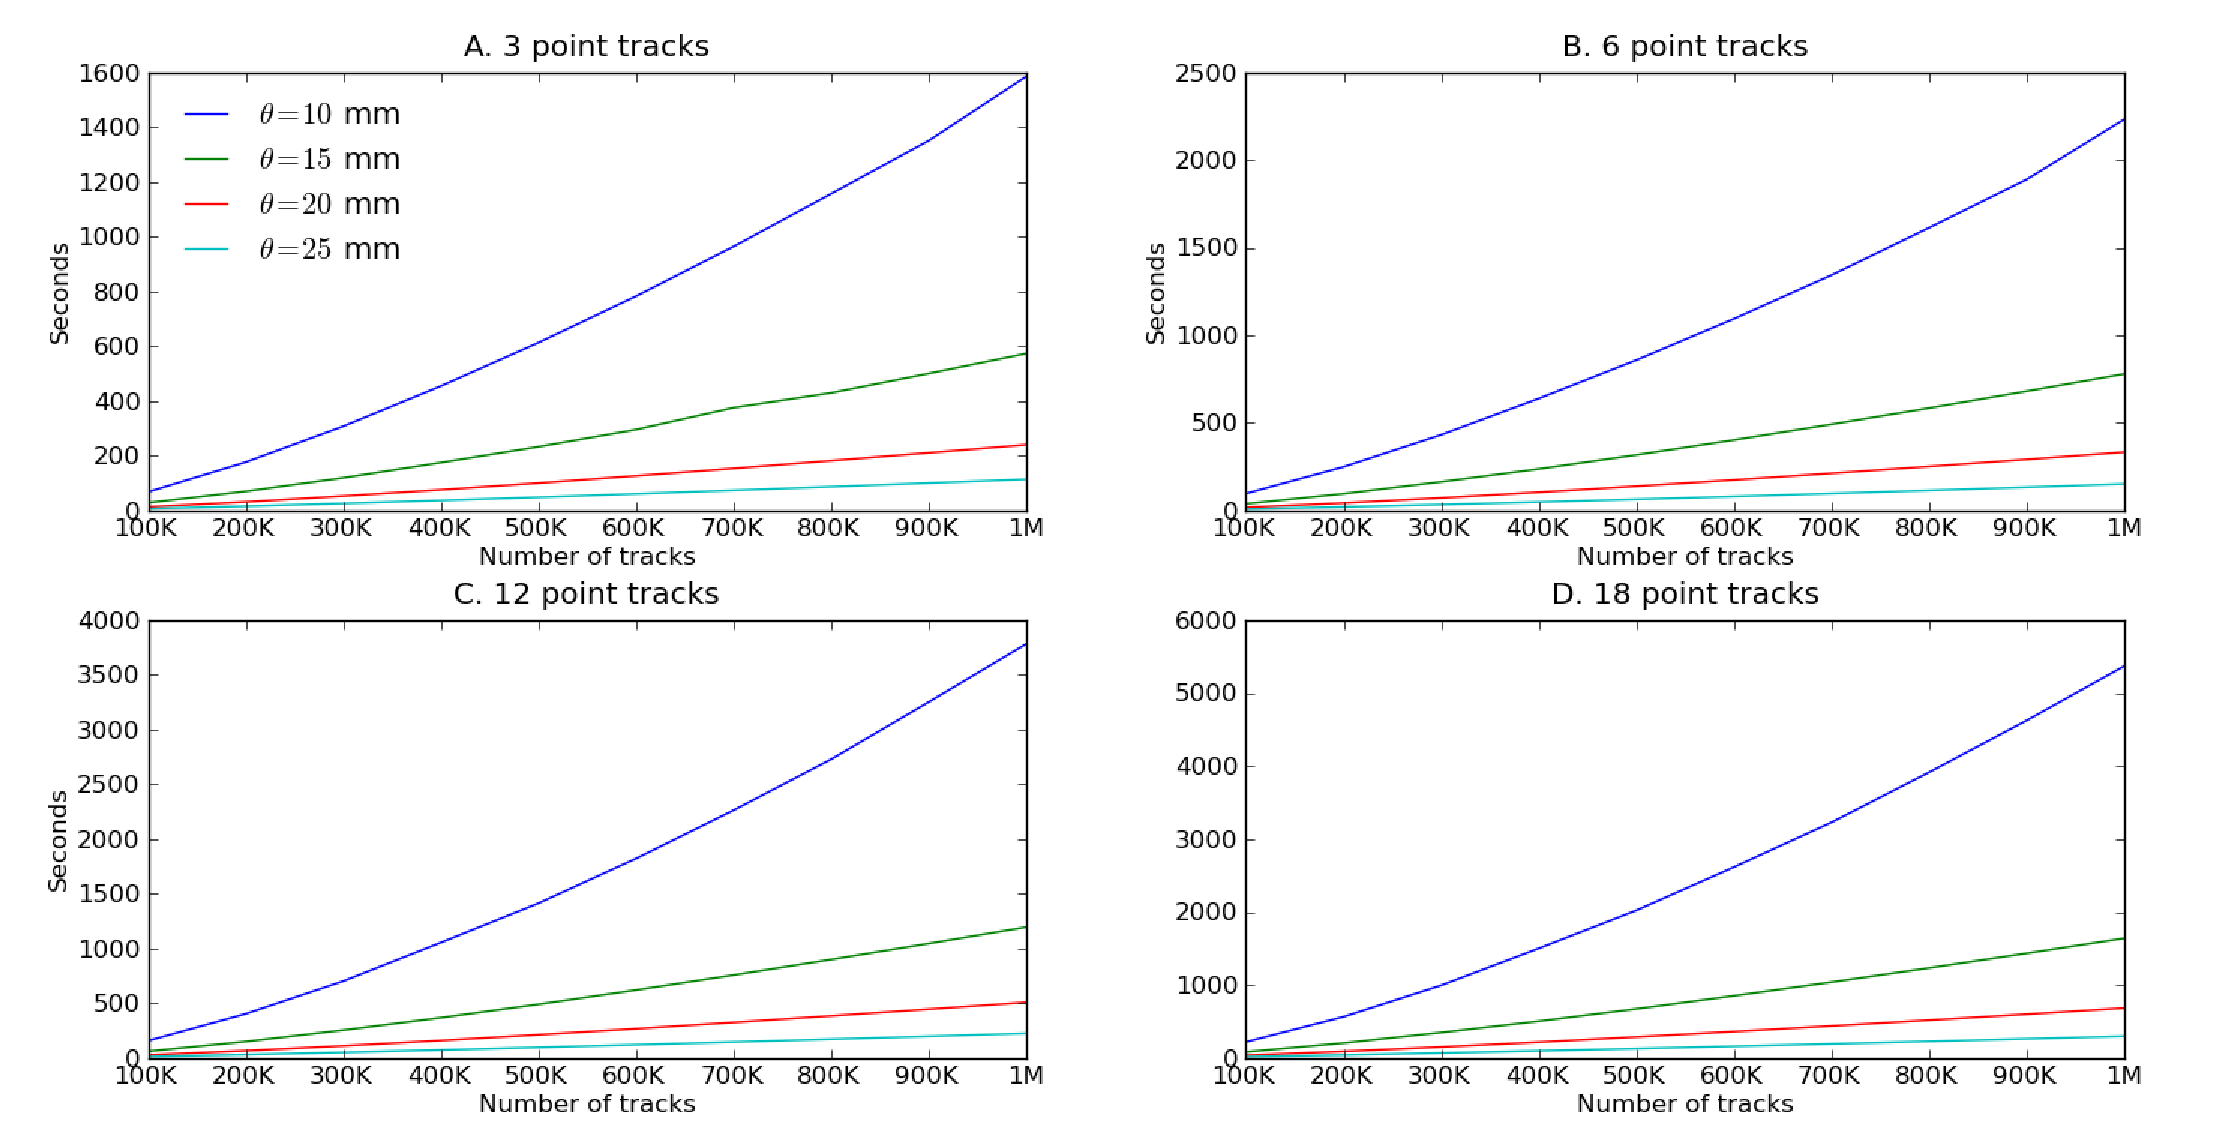
\includegraphics[scale=0.33]{Fig_3_2x2+leg-box}
\par\end{centering}
\caption{Time comparisons of QB using different number of points per
  track, different distance thresholds and different number of
  tracks. QB is a very efficient algorithm whose performance is
  controlled by just three parameters. (1) the initial downsampling $K$
  of the tracks exemplified in four sub-diagrams: 3 points (A), 6 points
  (B) 12 points (C), 18 points (D). (2) the distance threshold $\theta$
  in millimeters shown in 4 colours: 10~mm (blue), 15~mm (green), 20~mm
  (red), 25~mm (cyan). The final parameter, not shown explicitly in
  these diagrams, is the underlying structure of the data which is
  expressed by the resulting number of clusters.  We used a full
  tractography to generate these figures without removing or
  preselecting any parts. (NB The sub-diagrams use
  different vertical scales.) Random subsets of the tractography were
  chosen with size $N$ from \numrange{e5}{e6} (x-axis)\label{Flo:Speed1}}
\end{figure}

\subsection{Stability of QB\label{sub:Comparisons}}

One of the disadvantages of most clustering algorithms is that they give
different results with different initial conditions; for example this is
recognised with k-means, expectation-maximization
\citep{dempster1977maximum} and k-centers \citep{gonzalez1985clustering}
where it is common practice to try a number of different random initial
configurations. The same holds for QB so if there are not distinct
clusters such that the distance between any pair of clusters is
supra-threshold, then with different permutations of the same
tractography we will typically see similar number of clusters but
different underlying clusters. We will examine the robustness of QB in
this respect in section \ref{sub:Comparisons}.

As a first step towards examining the robustness of QB in this respect
we recorded the numbers of QB clusters in $20$ different random
orderings of the tractographies of $10$ human subjects acquired as
described in section \ref{sub:QB-Data-sets}. We removed short tracks
shorter than $40$~mm and downsampled the tracks at $12$ points. Then we
applied QB with threshold at $10$~mm. The mean number of clusters was
$2645.9$ (min $1937.6$; max $3857.8$; s.d.~$653.8$). There is therefore
a considerable between-subject variation in this metric. By contrast the
within-subject variability of the number of clusters across random
orderings is rather small, with mean standard deviation $12.7$ (min
$7.3$; max $17.4$). This suggests an encouraging level of robustness in
terms of the numbers of clusters that QB creates.

We ran an experiment were we evaluated TC~(\ref{eq:TC}) between pairs of
$10$ subjects with their tractographies warped in MNI space. This
generated $45$ TC values with $\theta=10$~mm. We did
this experiment twice; first by keeping only the bundles with more than
$10$ tracks (TC10) and secondly by keeping only the bundles with more
than $100$ tracks (TC100). The average value for TC10 was $47\%$ and
standard deviation $2.6\%$. As expected TC100 (bigger landmarks) did
better with average value of $53\%$ and standard deviation $4.9\%$. The
difference between TC10 and TC100 is highly significant: Student's
t$=4.692$, df=88, $p=1.97\times10^{-5}$, two-sided; and, as a precaution
against non-normality of the underlying distributions, Mann-Whitney U =
530., $p=5.65\times10^{-5}$. If we think that the small bundles of size
$<100$ are more idiosyncratic or possibly more likely to reflect noise
in the data, whereas larger bundles are more indicative of substantial
structures and landmarks in the tractographies, then we are encouraged
to see that on average the virtual tracks of $50\%$ of larger bundles of
each tractography lie within $10$~mm of those of the other
tractographies. This supports the notion that QB can be used to find
agreements between different brains by concentrating on the larger (more
important) clusters. We will see further evidence for this below
(section \ref{sub:Atlases-made-easy}).

As a further test we compared QB with $12$ point tracks and distance
threshold at $\theta=10$~mm versus some timings reported from other
state of the art methods found in the literature (Table
\ref{Flo:timings}). Unfortunately timings were very rarely reported up
till now as most algorithms were very slow on full data sets. This
experiment was performed using a single CPU core. Nonetheless the
speedup that QB offers is obviously of great importance and holds out
the prospect of real-time clustering on data sets of fewer than $20,000$
tracks (see Table~\ref{Flo:timings}).

%
\begin{table}
\small\addtolength{\tabcolsep}{-5pt}

\begin{centering}
\begin{tabular}{ccccc}
\hline 
\hline
Number of tracks ($N$) & Algorithms & Timings (secs) & QB (secs) & Speedup\tabularnewline
\hline
$1000$ & \citet{wang2010tractography} & $30$ & $0.07$ & $429$\tabularnewline
$60,000$ & \citet{wang2010tractography} & $14400$ & $14.7$ & $980$\tabularnewline
$400,000$ & \citet{Visser2010} & $75000$ & $160.1$ & $468$\tabularnewline
\hline
\end{tabular}
\par\end{centering}
\caption{Performance timings for QB run on $K=12$ point tracks and
  distance threshold at $\theta=10$~mm compared with some timings
  reported from other state of the art methods found in the
  literature. Unfortunately timings were very rarely reported until now
  as most algorithms were very slow on full data sets. Nonetheless, we
  can observe in this table that the speedup offered by QB offers is
  substantial.\label{Flo:timings}}
\end{table}

\subsection{The QB Sketch}

One of the major benefits of applying QB to tractographies is that it
can provide meaningful simplifications and find structures that were
previously invisible or difficult to locate because of the high density
of the tractography. For example we used QB to cluster the corticospinal
tract (CST). This bundle was part of the data sets provided by the
Pittsburgh Brain Competition (PBC2009-ICDM) and it was selected by an
expert. The QB Sketch is clearly shown in Fig.\ref{Flo:cst_pbc} where
every cluster is represented by a single virtual track. To generate this
clustering we used a tight threshold of $10$~mm. We observe that only a
few virtual tracks travel the full distance from bottom to top and that
they are many tracks that are broken (i.e. shorter than what was
initially expected) or highly divergent.

%
\begin{figure}
\begin{centering}
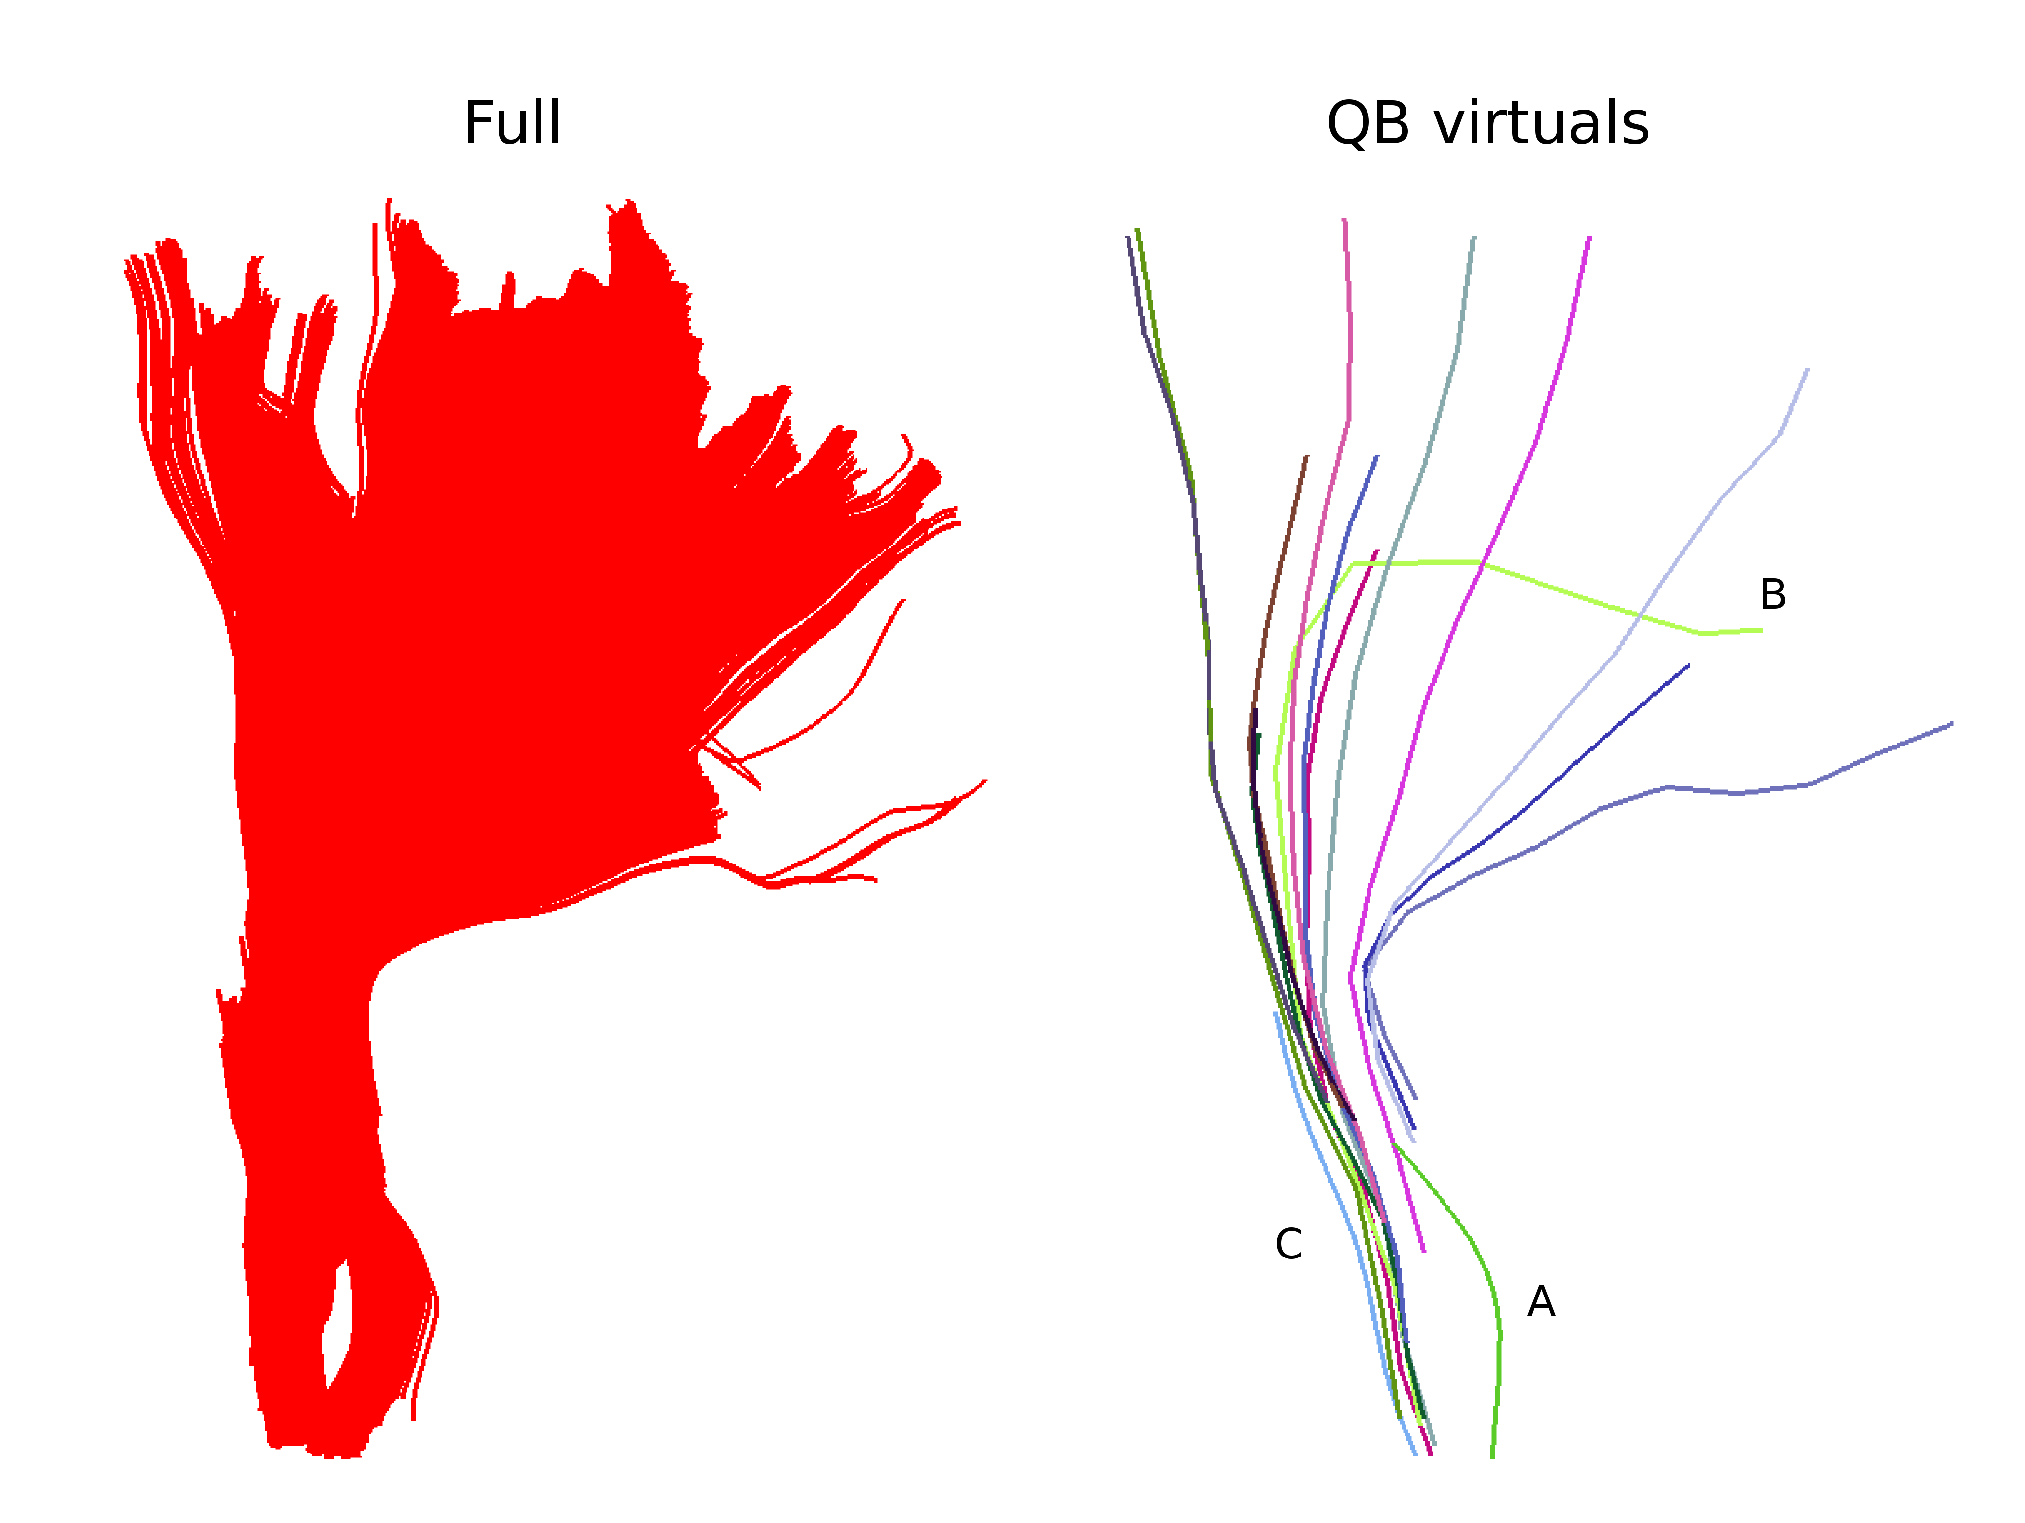
\includegraphics[scale=0.3]{Fig_4_cst_simplification}
\par\end{centering}
\caption{On the left the CST bundle is shown (red) consisting of $11041$
  tracks which were merged by an expert (PBC2009 data). At first glance
  it looks as though all tracks have a similar shape, and possibly
  converge towards the bottom, and fan out towards the top. However,
  this is a misreading caused by the opaque density when all the tracks
  are visualised.  QB can help us see the fuller structure of the bundle
  and identify its elements. On the right hand side we see the 14 QB
  virtual tracks of the CST generated by running QB with distance
  threshold of $10$~mm after downsampling to $12$ points. We can now
  clearly see that lots of parts which looked homogeneous are actually
  broken bundles e.g. dark green (A), light blue (C) or bundles with
  very different shape e.g. light green virtual track (B). To cluster
  this bundle took $0.135$~s.\label{Flo:cst_pbc}}
\end{figure}

Another interesting feature of QB is that it can be used to merge or
split different structures by changing the distance threshold.  This is
shown in Fig.~\ref{Flo:simulated_orbits}; on the left we see simulated
paths made from simple sinusoidal and helicoidal functions packed
together. The colour coding is used to distinguish the three different
structures. With a lower threshold the three different structures remain
separated but when we use a higher threshold the red and blue bundles
are represented by only one cluster indicated by the purple virtual
track.

\begin{figure}
\begin{centering}
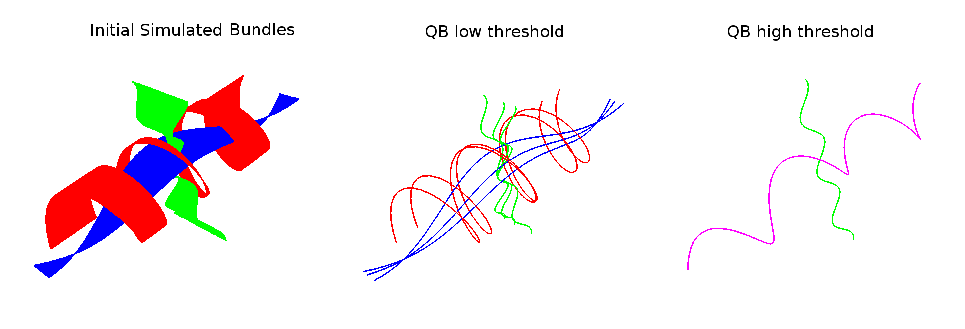
\includegraphics[scale=0.7]{Fig_5_helix_phantom}
\par\end{centering}
\caption{On the left we see $3$ bundles of simulated trajectories; red,
  blue and green consisting of $150$ tracks each. All $450$ tracks are
  clustered together using QB and the virtual tracks are shown when
  threshold $1$ was used shown in the middle and $8$ on the right.  We
  can see that when the threshold is low enough the underlying structure
  is a more detailed representation of the underlying geometry. However,
  when the distance threshold is higher, closer bundles could merge
  together as seen in the result on the right panel where the red and
  blue bundle have merged together in one cluster represented by the
  purple virtual track.\label{Flo:simulated_orbits}}
\end{figure}

Similarly, with the simulations shown in Fig.\ref{Flo:simulated_orbits}
we can see the same effect on real tracks, e.g. those of the fornix
shown at the left panel of Fig.~\ref{Flo:QB_fornix} where we can obtain
different number of clusters at different thresholds. In that way we can
stress thinner or larger sub-bundles inside other bigger bundles. 

A full tractography containing $250,000$ tracks was clustered using QB
with a distance threshold of $10$~mm (Fig.~\ref{Flo:QB_fornix}).  We
produced a useful reduction of the initial tractography leaving only
$763$ virtual tracks. Bundles smaller than $10$ tracks were
removed. Every track shown here represents an entire cluster containing
from $10$ to $5000$ tracks each.

\begin{figure}
\begin{centering}
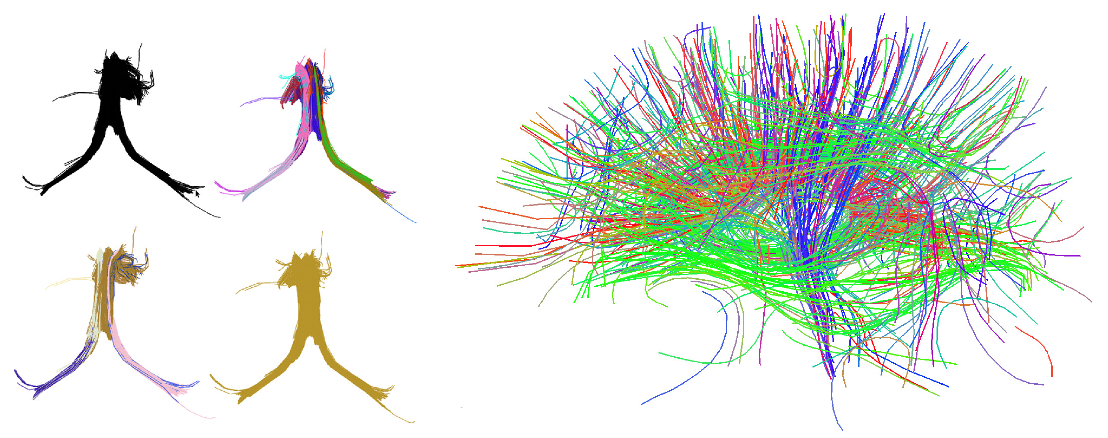
\includegraphics[scale=0.6]{Fig_6_QB_simple}
\par\end{centering}
\caption{Left panel: Here we see how QB clustered the fornix bundle with the
  data set from the PBC2009 competition. The original fornix is shown in
  black consists of $1076$ tracks. All tracks were equidistantly
  downsampled at $3$ points in this example. With a $5$~mm threshold our
  method generates $22$ clusters (top right). With $10$~mm generates $7$
  (bottom left) and with $20$~mm the whole fornix is determined by one
  cluster only (bottom right). Right panel: an example of a full tractography
  (\num{0.25e6} tracks) being clustered using QB with a distance threshold
  of $10$~mm. Here we see just $763$ virtual tracks depicted which
  produce a useful simplification of the initial tractography. Every
  track shown here represents an entire cluster from $10$ to $5000$
  tracks each. These can be thought as fast access points to explore the
  entire data set. The colour here just encodes track
  orientation.\label{Flo:QB_fornix}}
\centering{}
\end{figure}

The virtual tracks can be thought as fast access points to explore the
entire data set (see Fig.~\ref{Flo:QB_fornix}). With an appropriate
visualization tool we can click on a track and obtain the entire
cluster/bundle that it represents. Visualizing an entire data set of
that size is impossible on standard graphic cards and most visualization
tools e.g.~Trackvis (trackvis.org) or DSI Studio
(dsi-studio.labsolver.org) can only show a small random sample of the
full tractography at real time. In addition we have developed fast and
efficient ways of identifying broken or wandering tracks by using the
rapid data compression of QB to identify short or erratic virtual
tracks.

\subsection{Alignments, atlases and landmarks\label{sub:Atlases-made-easy}}

We have used QB to construct a robust tractographic atlas in MNI space
with data from 10 subjects. Here we explain the steps we used to achieve
this.

\textbf{Alignment}. Tractographies were created using EuDX as described
in section \ref{sub:QB-Data-sets}. The tractographies for all subjects
were initially in native space and the goal was to warp them in MNI
space, using nonlinear registration.

Because registration of brain anatomy between any two individuals is generally
considered a difficult problem with a non-unique solution we wanted to make sure
that we are using a known, well established and robust method, therefore we
chose to use $\texttt{fnirt}$ with the same parameters as used with the initial
steps of TBSS~\citep{Smith2006NeuroImage}. For that reason FA volumes were
generated from the same data sets using Tensor fitting with weighted least
squares after skull stripping with $\texttt{bet}$ and parameters $\texttt{-F -f
.2 -g 0}$. These FA volumes were again in native space therefore we needed to
warp them in MNI space. For this purpose a standard template
($\texttt{FMRIB58\_FA\_1~mm}$) from the FSL toolbox was used as the reference
volume. However, we wanted primarily to have the displacements which would do a
pointwise mapping from native space to MNI space and we found this to be
technically very difficult with the FSL tools as they assume that these
displacements will be applied only on volumetric data and not with point data as
those used in tractographies. We found a combination of $\texttt{flirt}$,
$\texttt{invwarp}$, $\texttt{fnirtfileutils}$ and $\texttt{fnirtfileutils
-withaff}$ which gave us the correct displacements. As this being very technical
we will not describe it further here but the code is available in our
$\texttt{Dipy}$ software package, in module ($\texttt{dipy.external.fsl}$). It
is important to note that we did not use eddy current correction with any of
this type of data sets. This correction is unstable with volumes acquired with
high b-values because there is not enough signal to guide a correct registration
with the other volumes at lower b-values.

The displacements estimated for every subject were applied
to each tractography in its native space, mapping it into MNI
space with voxel size $1\times1\times1~\textrm{~mm}^{3}$. Having all
tractographies in MNI space is especially useful because we can now
compare them against available templates or against each other and
calculate different statistics. However this is not where we stop; we
proceed to generate a tractographic atlas using QB clusterings.

\textbf{Tractographic Atlas:} For each subjects, (a) load the warped
tractography, (b) re-direct it towards a static point $(100,100,100)$, 
% as detailed in section~\ref{sub:The-bi-directionality-problem}, 
(c) downsample the tracks to have only $12$ points, and (d) calculate
and store QB clustering with a $10$~mm threshold. Then merge all
clusterings again with a $10$~mm threshold as explained in
section~\ref{sub:merging}. When creating an atlas by merging
many different subjects the most important issue is what one removes
from the atlas as outliers.  QB here provides a possible solution for
this problem. From the distribution of cluster sizes we find that $20\%$
of the largest clusters had more than $90\%$ of all tracks. This shows
that there is much agreement between the biggest bundles of different
subjects.  We will use this property to create a solid atlas in which we
keep the biggest bundles (landmarks) and remove small bundles
(outliers).

This atlas has been constructed without considering whether there are
inter-subject differences in white matter organisation. Outliers might
represent genuine differences in anatomy and the corresponding atlas
clusters can be explored to see how many subjects they relate to. With a
larger database QB can thus be used to create a probabilistic
tractography atlas with which to identify differences in morphology in
an analogous manner to that achieved for the cingulate and parasingulate
sulci by \citet{paus1996human}.

\textbf{Finding and Using Landmarks:} One can use this atlas or similar
atlases created from more subjects in order to select specific
structures and study these structures directly in different subjects
without using any of the standard ROI based methods.

A simple example is given in Fig.~\ref{Flo:CloseToSelected}. In the
first row we see a tractographic atlas joined by merging the QB
clusterings of $10$ healthy subjects as described in the previous
section. Then from these clusters represented by their virtual tracks we
keep only $196$ biggest clusters i.e. those which contain the highest
number of tracks, so that we are sure that there is enough agreement
from the different tractographies. From these we pick by way of an
example $19$ virtual tracks (see Tab.~\ref{Flo:structures} which
correspond to well known bundle structures in the literature:

\begin{table}
\small\addtolength{\tabcolsep}{-5pt}
\begin{centering}
\begin{tabular}{lll}
\hline 
\hline
Abbreviation & Structure \tabularnewline
\hline
GCC   & genu of corpus callosum \tabularnewline
BCC   & body of corpus callosum \tabularnewline 
SCC   & splenium \tabularnewline
CP    & pons cerebellar peduncle \tabularnewline
ARC-L & left arcuate fasciculus \tabularnewline
ARC-R & right arcuate fasciculus \tabularnewline
IFO-L & left inferior occipitofrontal fasciculus \tabularnewline
IFO-R & right inferior occipitofrontal fasciculus \tabularnewline
FX-R  & right fornix \tabularnewline
FX-L  & left fornix  \tabularnewline
OR    & optic radiation  \tabularnewline
CGL-L & left cingulum  \tabularnewline
CGL-R & right cingulum  \tabularnewline
CST-L & left corticospinal tract  \tabularnewline
CST-R & right corticospinal tract \tabularnewline
UNC-L & left uncinate \tabularnewline
UNC-R & right uncinate \tabularnewline
\hline
\end{tabular}
\par\end{centering}
\caption{19 virtual tracks chosen to represent 17 fibre bundles for 
  the analyses in Fig.~\ref{Flo:CloseToSelected}. Three tracks were 
  selected for BCC, all the other structures had one corresponding 
  track.\label{Flo:structures}}
\end{table}

These $19$ tracks are coloured randomly. Then on the second row we show,
for the first $6$ of these selected representative tracks, the tracks
closer than $20$~mm from $3$ arbitrarily selected subjects. Similarly,
on the third row the tracks closer than $15$~mm to the next $7$ selected
tracks. Finally on the last row we bring the tracks from the same $3$
subjects which are closer than $18$~mm.  The colours used for the
selected tracks are automatically assigned from the colours assigned to
the tracks picked from the atlas. We can see that there is a significant
reliability and continuity both within and between subjects even though
we have only selected a very small number of representative
tracks. Using a similar procedure we could create a list of bundles of
every subject and then compare the subjects at the level of bundles.

%
\begin{figure}
\begin{centering}
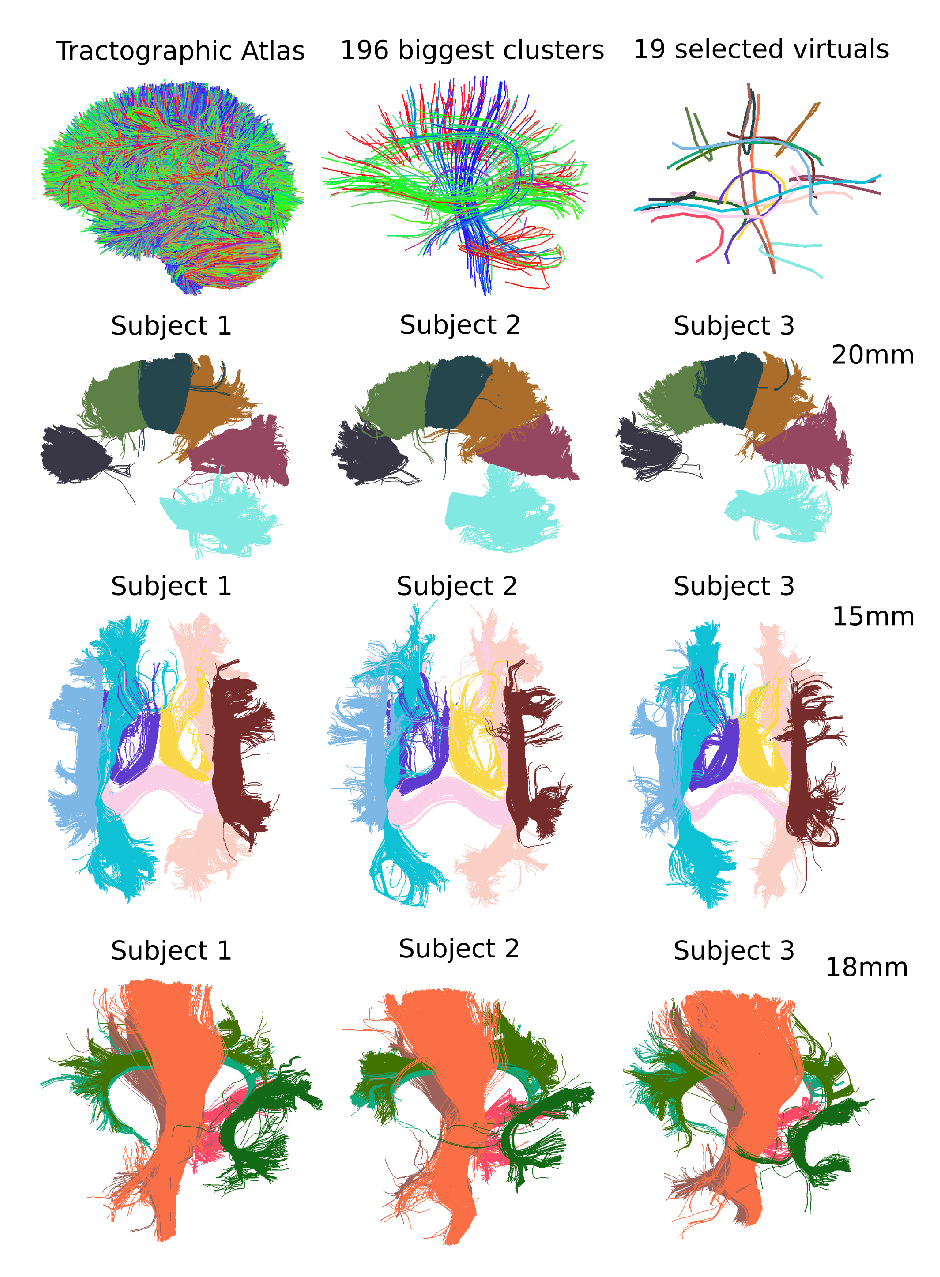
\includegraphics[scale=0.7]{Fig_7_close_distance}
\par\end{centering}
\caption{A novel way to do comparisons between subjects. Correspondence
  between different subjects (last $3$ rows) and a few landmarks picked
  from the tractographic atlas generated by merging QB clusterings of
  $10$ subjects (top row). The fact hat we can see this amount of
  agreement and continuity on the last $3$ rows from such a few virtual
  tracks raises the hope of implementing new robust ways of statistical
  comparisons using tractographic data sets.\label{Flo:CloseToSelected}}
\end{figure}

\subsection{QB as input to other clustering methods}

We found that QB is of great value as an adjunct to many less efficient
algorithms e.g. hierarchical clustering, affinity propagation, nearest
neighbours, spectral clustering and other unsupervised and supervised
machine learning methods. We present here one example with QB as input to
affinity propagation and one with QB as input to hierarchical
clustering.

Most clustering algorithms need to calculate all pairwise distances
between tracks; that means that for a medium sized tractography of
\num{250000} tracks we would need $232$ GBytes of RAM with single floating
point precision. Something which is not and will not be available soon
in personal computers. In those cases some people might hope that sparse
matrices could provide a nice approximation; however dense
tractographies produce very dense distance matrices. The straightforward
solution to this problem is to use QB in order to first segment in small
clusters and then use the representative tracks (i.e. exemplar or virtual
tracks) of these clusters with other higher complexity operations and merge the
clusters together in bigger clusters.

\textbf{Procedure}:

\begin{enumerate}

\item Cluster using QB as explained in section~\ref{sub:Atlases-made-easy}

\item Gather virtual tracks.

\item Calculate MDF distance of virtual tracks with themselves.

\item Use any other clustering method to segment this much smaller distance
matrix $D$.

\end{enumerate}

In the left panel of Fig.~\ref{Flo:LSC+HC+AP} we show a result where we
used hierarchical clustering with single linkage for step (4) with a
threshold of $20$~mm using the Python software package
$\texttt{hcluster}$~\citep{eads-hcluster-software}. A known drawback of
single linkage is the so-called chaining phenomenon: clusters may be
brought together due to single elements being close to each other, even
though many of the elements in each cluster may be very distant to each
other. Chaining is usually considered as a disadvantage because it is
too driven by local neighbours. Nevertheless, we can take advantage this
property to cluster the entire corpus callosum (CC) together (shown in
dark red in left top of Fig.~\ref{Flo:LSC+HC+AP}) creating a fully
automatic CC detection system.  Furthermore, we can use different
cutting thresholds on the underlying dendrogram to amalgamate together
different structures (see e.g.~the cingulum bundles in the same panel).

In the right panel of Fig.~\ref{Flo:LSC+HC+AP} we see an implementation
of step (4) using the more recent algorithm, affinity propagation
(AP)~\citep{dueck2009affinity}, which has been
identified~\citep{malcolm2009filtered}) as being difficult or impossible
to be used for group analysis or to cluster entire tractographies of
many thousands of tracks.
% A small outline
% of how this algorithm works is given in section \ref{sub:Affinity-Propagation}.
Here we see in the bottom right panel of (see Fig.\ref{Flo:LSC+HC+AP})
how nicely AP, after the simplification provided by QB, has clustered
arcuate, longitudinal occipitofrontal fasciculus and other structures
known from the literature. The input of AP was the negative distance
matrix $-D$, the preference weights were set to matrix $\mathtt{median}(-D)$
and the hierarchical clustering parameter was set to $20$~mm.
For affinity propagation we used the Python library \texttt{scikit-learn}.

\begin{figure}
\begin{centering}
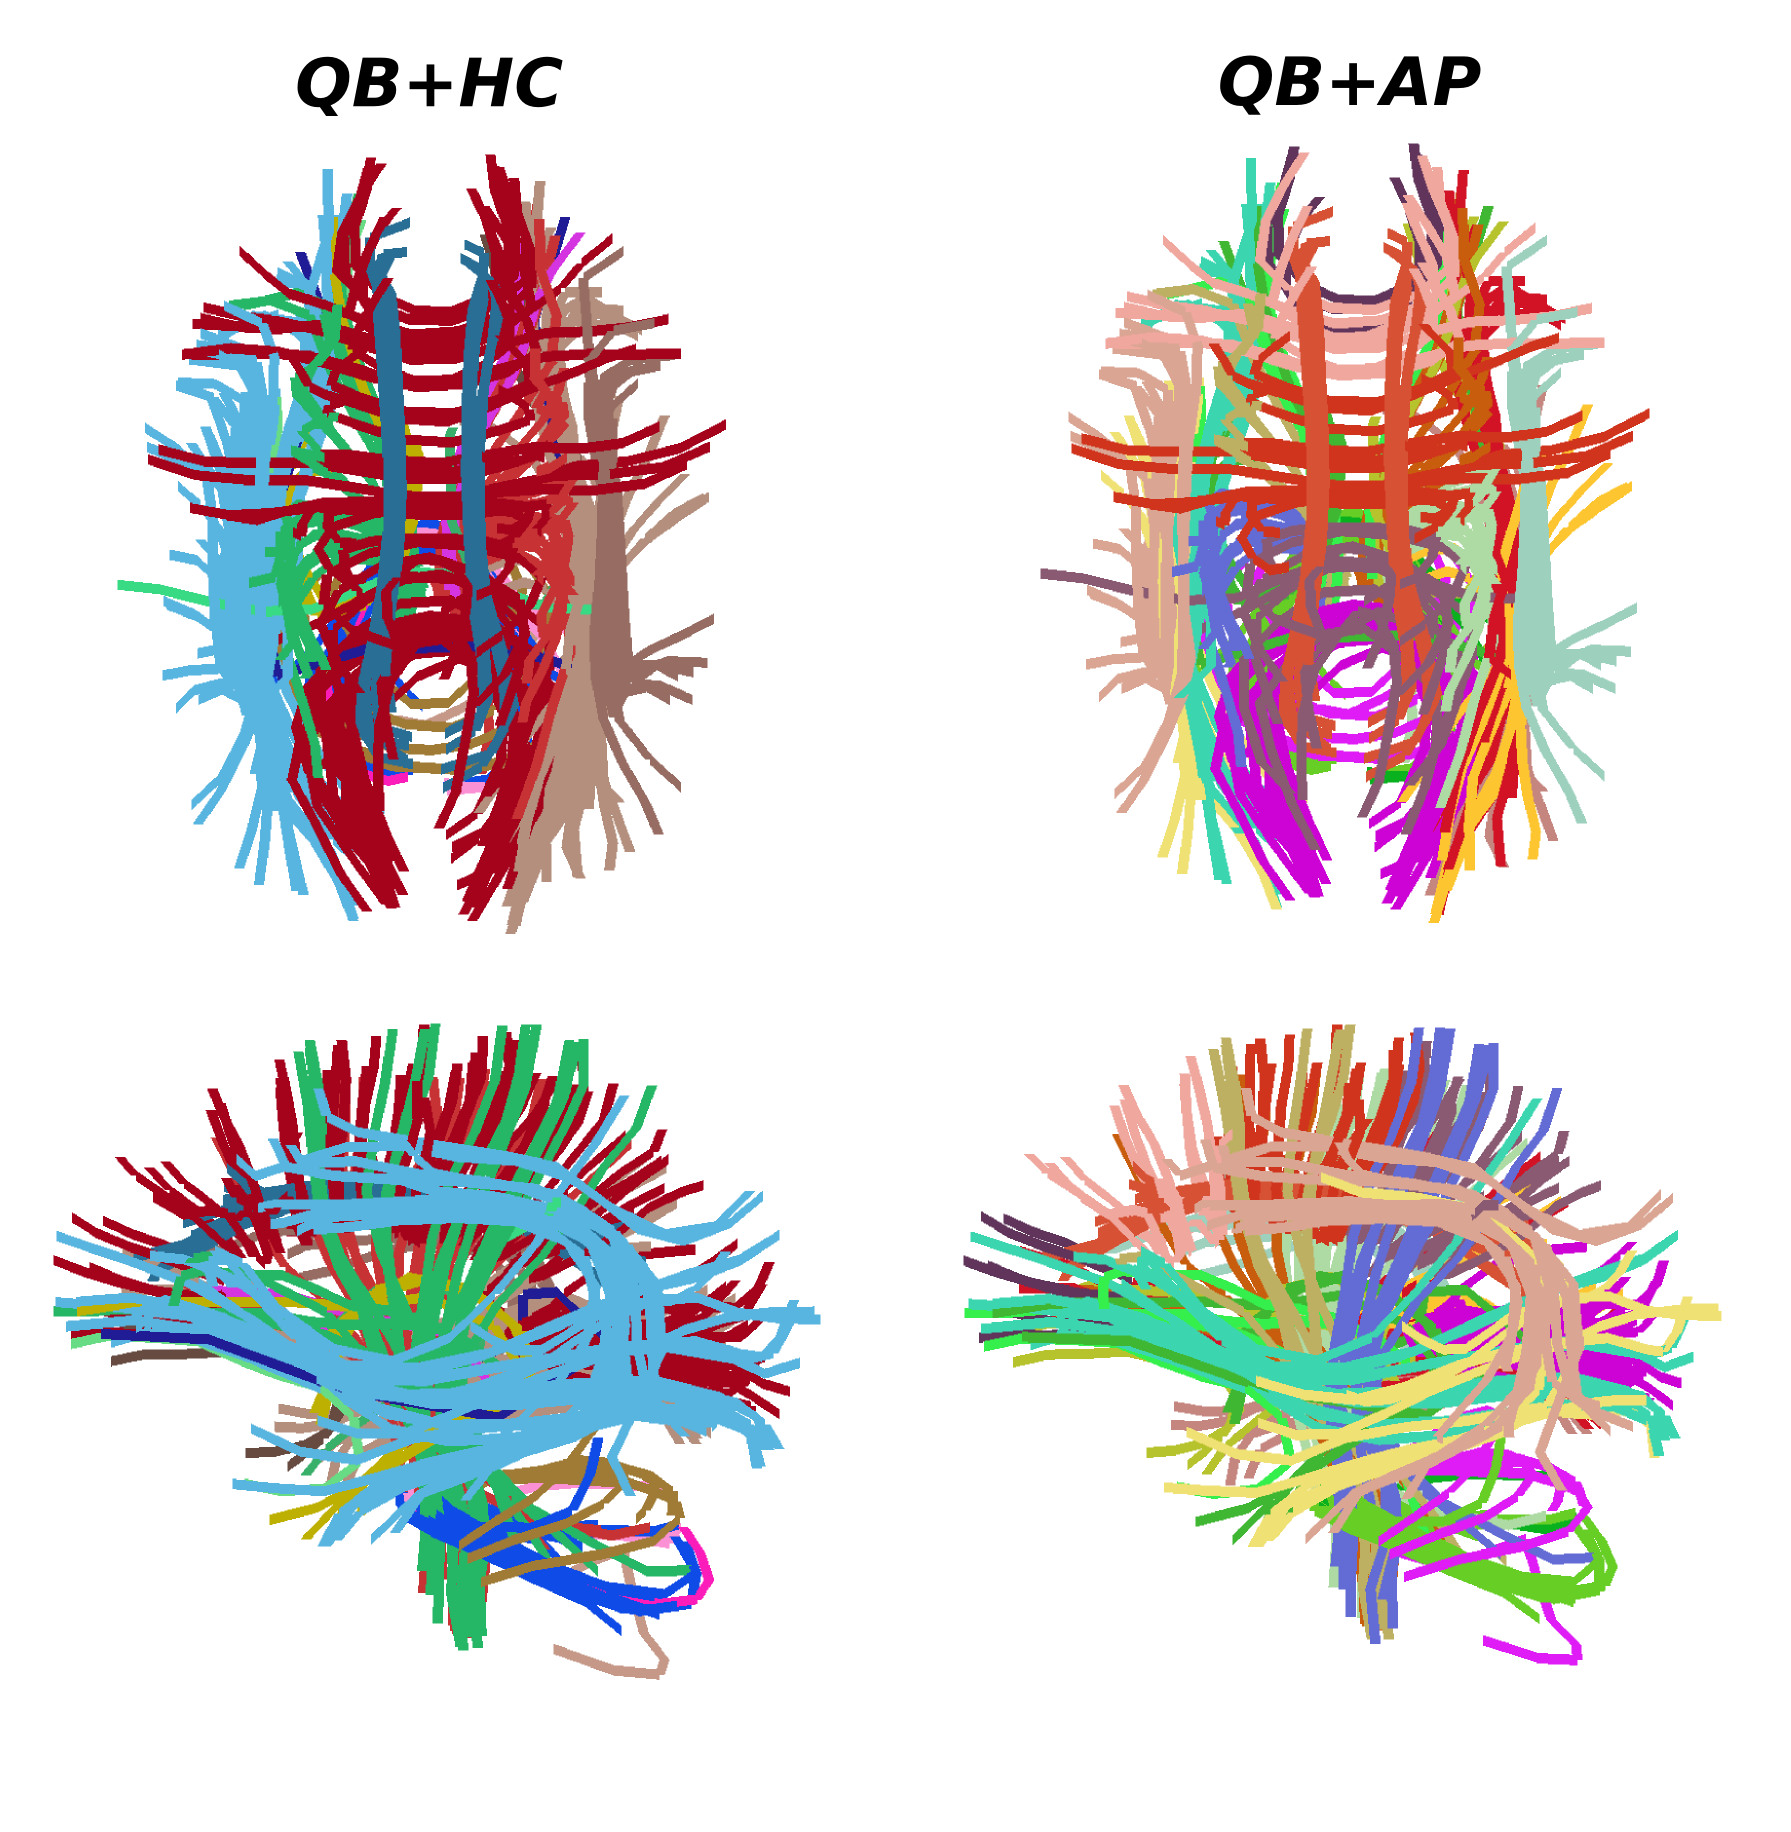
\includegraphics[scale=0.7]{Fig_8_QB_with_others}
\par\end{centering}
\caption{Two examples where QB output is used to cluster an entire set
  of $10$ tractographies together and then the result is given as input
  to hierarchical clustering (HC) using single linkage on the left and
  to affinity propagation (AP) on the right. Colours encode cluster
  labels. On the left side we see 19 clusters and on the right 23. QB
  facilitates significantly the operation of the other two algorithms
  which would not be able to cluster the entire data sets on current
  computers. Note the top left panel where QB+HC have managed to cluster
  the entire CC in one bundle.\label{Flo:LSC+HC+AP}}
\end{figure}

While clustering methods of higher order complexity such as HC and AP
have considerable theoretical appeal and have a deserved reputation for
being able discover meaningful structure in data sets they are simply
impracticable when more than a few thousand items are being
clustered. Using QB to pre-process the tractography puts the whole data
set, condensed to its virtual tracks, within the feasible range of these
higher order algorithms.

\subsection{Exemplars improve on use of ROIs or masks}

Medical practitioners and neuroanatomists often argue that when they use
multiple spherical or rectangular masks to select some bundles many
tracks are thrown away because they are small and the mask operations
cannot get hold of them. Our method provides a solution to this problem
as it can identify broken or smaller bundles inside other bigger bundles
which are otherwise very difficult or even sometimes impossible to
identify visually or with the use of masks. Our method attacks this
problem and suggests a very efficient and robust solution which sets the
limit for unsupervised clustering of tractographies and facilitates
tractography exploration and interpretation. The point here is that one
can now use exemplar tracks as access points into the full tractography
and with a single click on that exemplar track obtain the entire bundle.
Therefore a super-bundle can be created just with with a few clicks
based on a selection from exemplar tracks.

In order to create this system we implemented a 3D
visualization/interaction system for tractographies based on QB in
Python and OpenGL. This code is available online at fos.me.


\subsection{Direct Tractography Registration}

Direct tractography registration is a recently described problem with
only a small number of publications \citep{leemans2006multiscale,
  mayer2008bundles, mayerdirect, mayer2011supervised,
  durrleman2010registration, zvitia2008adaptive, Zvitia2010,
  ZiyanMICCAI07}, and so far as we know there are no publicly available
solutions. By direct registration we mean that no other information
apart from the tractographies themselves is used to guide the
registration. This is in contrast to
section~\ref{sub:Atlases-made-easy}) where we used FA registration
mappings applied to tractographies which is also most commonly used in
the literature along with other Tensor based
methods~\citep{goh2006algebraic}.

We now describe our algorithm which is efficient and simple
to use, completely automatic and provides an evidently robust direct
rigid tractography registration algorithm available in seconds. This
algorithm could be of great use when comparing healthy versus severely
diseased brains e.g.~stroke or vegetative state patients when non-rigid
registration is not recommended because of severe asymmetries in the
diseased brains. The algorithm is based on the robustness of QB to find
good representative descriptors.

\textbf{Procedure}. Here we describe a simple algorithm where $2$
tractographies $T_{A}$,$T_{B}$ are brought into alignment in native
space.
\begin{enumerate}
\item All tracks with length smaller than $100$~mm and longer than $300$~mm
are removed from the data sets. This will reduce the size of tractography
to about $1/4$ of its initial size (\textasciitilde200,000 tracks). (While all
the subjects are adults, this filtering may have different effects
depending on brain size. We have not investigated this question at
present.)
\item Both tractographies are equidistantly downsampled so every track contains
only $12$ points. 
\item We run QB with distance threshold at $10$~mm for both tractographies.
\item Collect all exemplar tracks from clusters containing more than $0.2\%$
of all tracks. Let us assume we have these now in $E_{A}$ and $E_{B}$.
\item Calculate all pairwise distances $D=\mathtt{MDF}(E_{A},E_{B})$ and
save them in rectangular matrix $D$. 
\item Create a cost function (optimizer) which we will try to minimize the
symmetric minimum distance $\mathrm{SMD}=\sum_{i}\min_{j}D(i,j)+\sum_{j}\min_{i}D(i,j).$
\item Use modified Powell's method \citep{fletcher1987practical} to minimize
$\mathrm{SMD}$ over rigid rotations of $E_{\mathcal{B}}$ starting
with zeroed initial conditions. At each iteration of the optimization,
$E_{B}$ will be transformed by a rigid rotation and $\mathrm{SMD}$
will be recalculated. To ensure smooth rotations we use the Rodriguez
rotation formula.
\end{enumerate}

In Fig.\ref{Flo:direct_registration} A we see the result of this
algorithm applied to two tractographies represented by their
exemplar tracks, depicted in orange and purple. We can see in the
upper panel that the orange tractography is misaligned with respect to
the purple one, and in the lower panel we see their improved alignment
after applying our algorithm.

\textbf{Metric}. SMD is proposed here for registration of trajectory
data sets, but one could equally use mutual
information~\citep{maes1997multimodality} or the correlation
ratio~\citep{roche1998correlation} for registration of volumetric data
sets. Nonetheless, the advantage of SMD is that it comes from robust
landmarks generated by QB which bring together local and global
components. Initially, it was not clear if we should use SMD or just the
sum of all distances $\mathrm{SD}=\sum_{i,j}D(i,j)$. Therefore, we made
a small experiment to validate the smoothness and convexity of these two
cost functions. We plotted both functions under a single-axis
translation or a single-angle rotation of the same tractography as show
in Fig.~\ref{Flo:direct_registration} B and C. From, these two diagrams
we can see that although for translations only the SD was entirely
convex, with rotations the SD had stronger local minima which is not a
good property for registration. Furthermore, the SMD had steeper
gradients towards the global minimum which is a positive indicator for
faster convergence.

\textbf{Experiments}. The first large scale experiment took place using
the same tractography of a single individual copied and transformed
$1000$ times with range of all three angles from \ang{-45} to \ang{45}
and range of all x,y,z translations from \numrange{-113}{113}~mm. Then
we registered all transformed tractographies to the static one and
calculated all pairwise MDF distances storing them in a square matrix
$D$. We would expect that if the registration was correct then the sum
of all diagonals elements of $D$ would be close to $0$. This was
confirmed with both cost functions used SD and SMD getting close to zero
$99.8\%$ of the time however SMD was always closer to perfect alignment
than SD. Consequently we chose SMD as a better cost function for direct
tractography registration.

We used GQI-based tractographies from $10$ subjects, and registered all
45 possible pairs. Comparing different tractographies is not a trivial
problem however we can use the tightness comparison (TC) metric
explained in section \ref{sub:Tightness-comparisons-1}.  We can report
that the mean initial TC was $34.8\%\pm8.0\%$ and the mean final TC
after applying our direct registration method was $48.1\%\pm6.1\%$. This
was a statistically highly significant improvement
($t_{\text{\textrm{paired}}}(44)=11.2$, $p\leq10^{-13}$ ). These TC
values are comparable to those reported in
section~\ref{sub:Tightness-comparisons-1}. We are planning in the future
to compare this registration method against other standard methods which
are common in the literature.

It should be noted that both TC and SMD are derived from the same
distance matrix $D_{AB}$ between the two sets of virtual
tracks. However, using TC to assess a registration that has minimised
SMD is less circular than might appear at first sight; the minimization
of SMD depends on all the entries of $D$ as it is the mean of all those
entries, while TC depends on the separate minimizations of the rows and
columns of $D$.

\begin{figure}
\begin{centering}
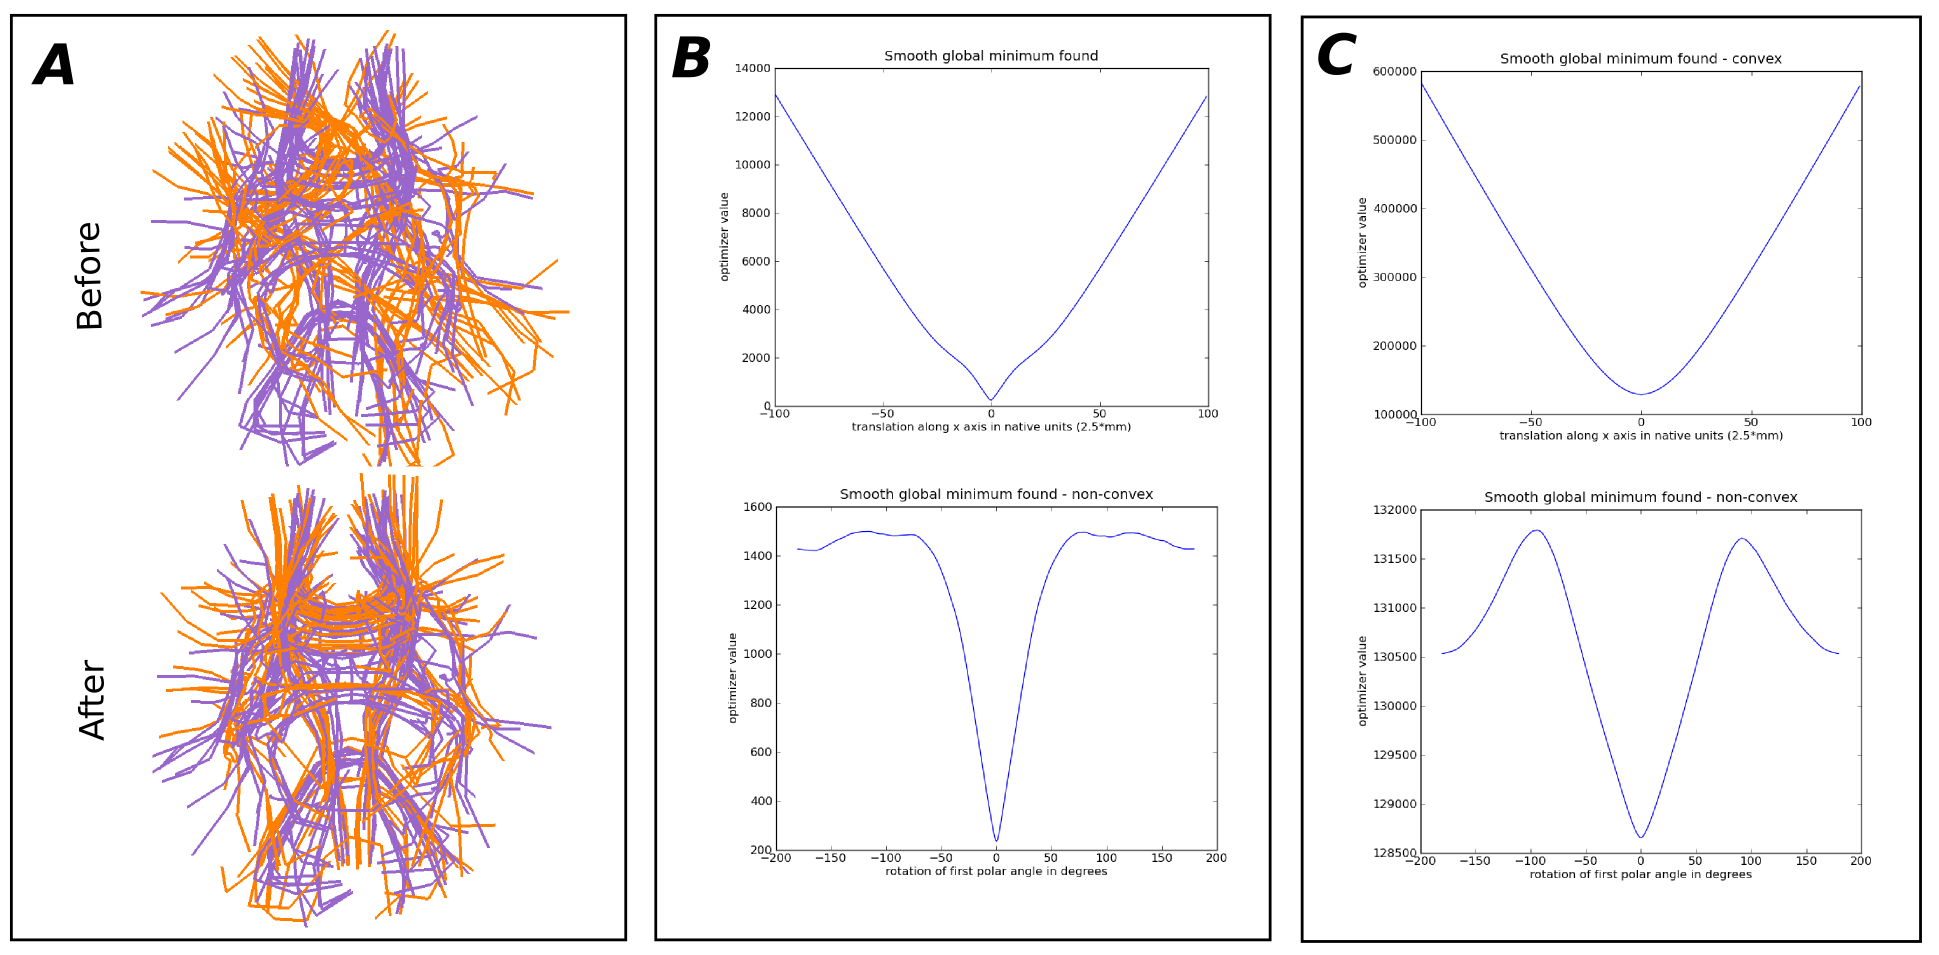
\includegraphics[scale=0.8]{Fig_9_QB_registration2}
\par\end{centering}
\caption{In panel A we see two tractographies from different subjects
  before (top) and after rigid registration (bottom) using our
  method. In panel B we see the metric $SMD$ that we chose to optimize
  for two copies of the same tractography with the second copy
  translated (above) and rotated (below). This metric appears to be
  smooth with a single global minimum and is only slightly non-convex
  with small local minima. In panel C another possible candidate metric
  $SD$ is shown which although more convex on translations it was much
  more problematic with rotations.\label{Flo:direct_registration}}
\end{figure}

\subsection{Strategies with short tracks}

We have not so far taken account of short tracks in this report. That
is perfectly valid because (a) the longer tracks are more likely to
be used as useful landmarks when comparing or registering different
subjects because it is more likely for them to exist in most subjects,
(b) removing short tracks facilitates the usage of distance based
clustering (no need for manually setting the distance threshold) and
interaction with the tractography, (c) typically one first wants to
see the overall representation of the tractography and later go to
the details. Nonetheless, after having clustered the longer tracks
there are many ways to assign the smaller bundles to their closest
longer bundles. For this purpose we recommend to use a different distance
from MDF for example the minimum version of MAM referred
to as $\textrm{MAM}_{\textrm{min}}$ in Eq.~(\ref{eq:minimum_distance}). 

%
\begin{figure}
\begin{centering}
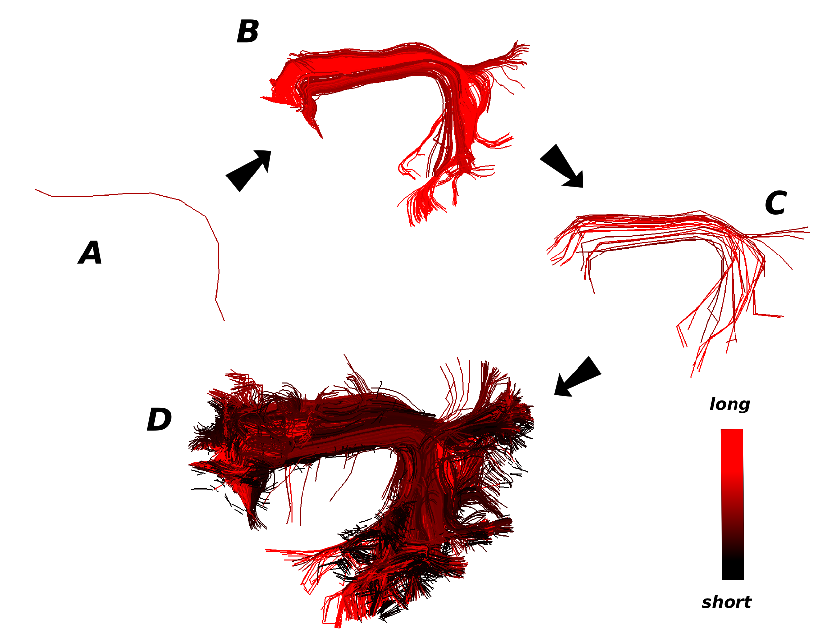
\includegraphics[scale=0.7]{Fig_10_arcuate_small_fibers}
\par\end{centering}
\caption{A simple and vigorous strategy for handling short and long
  tracks together by picking a track of interest from one of our
  atlases. Colour map here encodes track length. A: a single selected
  atlas track, B: for a single subject, $245$ actual tracks closer than
  $15$~mm (MDF distance), C: the tracks from B clustered with $23$
  virtual tracks, D: $3421$ actual tracks closer than $6$~mm
  ($\textrm{MAM}_{\textrm{mean}}$ distance) from the virtual tracks in C
  are shown. We can see that a great number of short tracks have been
  brought together along with the tracks in B. In this way we managed to
  bring together an entire bundle consisting both of long and short
  tracks by just selecting one track.\label{Flo:arcuate_close}}
\end{figure}

Here we show some simple strategies for clustering short fibres. The first
is for unsupervised clustering and the second one is for supervised
learning.

\textbf{Strategy 1:} Cluster the long tracks using QB with distance
threshold at $10$~mm and then cluster the short tracks (<$100$~mm) to a
lower threshold and assign them to their closest long track bundle from
the first clustering using the $MAM_{min}$ distance.

\textbf{Strategy 2:} Read the tractography of a single subject, use a
tractographic atlas as the one created in
section~\ref{sub:Atlases-made-easy} and pick one or more close virtual
tracks from that atlas and then find the closest tracks from the subject
to that selected track using $d_{df}$, cluster the closest tracks found
from the previous step and for each one of these new virtual tracks find
the closest tracks using the $m_{in}$. We should now have an
amalgamation of shorter and longer tracks in one cluster.

An example of this second strategy is shown in
Fig.~\ref{Flo:arcuate_close}: (A) a track of interest from the arcuate
fasciculus is selected from the tractographic atlas shown in
Fig.~\ref{Flo:CloseToSelected} (top row, centre), (B) the tracks of the
subject closer than 15~mm ($d_{df}$) from the selected cluster are shown
and clustered with a distance threshold of $6.25$~mm in (C), (D) from
every virtual track in C we find the closest tracks using the
($m_{in}$) distance from the entire tractography.

\section{Discussion and conclusion}

We have presented a novel and powerful algorithm -- QuickBundles
(QB). This algorithm provides simplifications to the old problem of
revealing the detailed anatomy of the densely packed white matter which
has recently attracted much scientific attention; it can also be used
for any trajectory clustering problem and it is recommended when large
data sets are involved. QB can be used with all types of diffusion MRI
tractographies which generate streamlines (e.g. probabilistic or
deterministic) and it is independent of the reconstruction model.

In common with mainstream clustering algorithms such as k-means,
k-centers and expectation maximization, QB is not a global clustering
method therefore it can give different results under different initial
conditions of the data set when there is no obvious distance threshold
which can separate the clusters into meaningful bundles; for example we
should expect different clusters under different permutations/orderings
of the tracks in a densely packed tractography. However, we found that
there is enough agreement even between two clusterings of the same
tractography with different orderings. If the clusters are truly
separable by distances then there is a global solution independent of
orderings. This is often visible in smaller subsets of the initial
tractography. We empirically found that this problem is minimized even
with real data sets when a low distance threshold of about $10-20$~mm is
used.

Furthermore the output of QB can be used as the input to another recent
fast algorithm of quadratic time on average $\mathcal{O}(M^{2})$ called affinity
propagation where now $M\ll N$ therefore the overall time stays linear
on the number of tracks $N$. Other algorithms previously too slow to be
used on the entire tractography can now be used efficiently too
e.g.~k-nearest neighbour (k-NN), and hierarchical clustering.

We saw that QB is a linear time clustering method based on track
distances, which is on average linear time $\mathcal{O}(N)$ where $N$ is
the number of tracks and with worst case $\mathcal{O}(N^{2})$ when every
track is a singleton cluster itself. Therefore QB is the fastest known
tractography clustering method and even real-time on smaller
tractographies (<20,000 tracks). We also showed that is uses a negligible amount of
memory.

QB is fully automatic and very robust as when we use it we can find good
agreements even between different subjects and can be used to create
tractography atlases at high speed. Additionally, it can be used to
explore multiple tractographies and find correspondences between
tractographies, create landmarks used for registration or population
comparisons.

QB can be used as well for reducing the dimensionality of the data sets
at the time of interaction providing an alternative way to ROIs using
BOIs (bundles of interest). We also showed
that it can be used to find obscured tracks not visible to the user
at first instance. Therefore QB opens up the road to create a rapid
tools for exploring tractographies of any size.

We have shown results with data from simulations, and single and
multiple real subjects. The code for QuickBundles is freely available at
dipy.org.

\section{References}

\selectlanguage{british}%
\bibliographystyle{elsarticle-harv}
\bibliography{QB_NeuroImage}
\selectlanguage{english}

\begin{appendices}
\numberwithin{equation}{section}
\numberwithin{algorithm}{section}

\section{The QB algorithm\label{Sec:QB-Algorithm}}

\subsection{Formal specification\label{sub:QB-specification}}

The QB algorithm was described in section~\ref{sub:QB-description}. A formal
specification is given in Algorithm~\ref{Alg:QuickBundles}.

\begin{algorithm}
\textbf{Input:} tracks $T=\{s_{0},...,s_{i},...,s_{|T|-1}\}$, threshold $\theta $\\
\textbf{Output:} clustering $C=\{c_{0},...,c_{k},...,c_{|C|-1}\}$ where cluster $c=\{I,\mathbf{h},N\}$\\
\\
$c_{0}=\left\{0,s_{0},1\right\}$\\
$C=\left\{c_{0}\right\}$ \# the first track becomes the first cluster\\
$|C|=1$ \# the total number of clusters is 1 \\
$\textbf{For}$ $i$ $\textbf{From}$ $1$ $\textbf{To}$ $|T|-1$ $\textbf{Do}$ \# all tracks\\
\hspace*{2em} $\textbf{t}=T_{i}$\\
\hspace*{2em} $\texttt{alld}=\textbf{0}$ \# distance buffer\\
\hspace*{2em} $\texttt{flip}=\textbf{0}$ \# flipping check buffer\\
\hspace*{2em} $\textbf{For}$ $k$ $\textbf{From}$ $0$ $\textbf{To}$ $|C|-1$ \# all clusters\\
\hspace*{4em} $\mathbf{v}=C_{k}.\mathbf{h}/C_{k}.N$\\ 
\hspace*{4em} $d$=$d_{\textrm{direct}}(\mathbf{t},\mathbf{v})$\\
\hspace*{4em} $f$=$d_{\textrm{flipped}}(\mathbf{t},\mathbf{v})$\\
\hspace*{4em} $\textbf{If}$ $f < d$ $\textbf{Then}$\\
\hspace*{6em} $d = f$\\
\hspace*{6em} $\texttt{flip}_{k} = 1$\\
\hspace*{4em} $\texttt{alld}_{k} = d$\\
$m=\min(\texttt{alld})$\\
$l=\mathrm{arg min}(\texttt{alld})$\\
$\textbf{If}$ $m < \theta$ \# append in current cluster \\
\hspace*{2em} $\textbf{If}$ $\texttt{flip}_{l}=1$ $\textbf{Then}$\\
\hspace*{4em} $C_{l}.\mathbf{h}+=t'$\\
\hspace*{2em} $\textbf{Else}$ \\
\hspace*{4em} $C_{l}.\mathbf{h}+=t$\\
\hspace*{2em} $C_{l}.N+=1$\\
\hspace*{2em} $C_{l}.I$.append($i$)\\
$\textbf{Else}$ \# create new cluster\\
\hspace*{2em} $|C|+=1$ \# total number of clusters increases\\
\hspace*{2em} $C_{|C|-1}.I_{0}=l$\\
\hspace*{2em} $C_{|C|-1}.\mathbf{h}=\mathbf{t}$\\
\hspace*{2em} $C_{|C|-1}.N=1$\\
\caption{QuickBundles\label{Alg:QuickBundles}}
\end{algorithm}

\subsection{Comparison with BIRCH\label{sub:BIRCH}}

QuickBundles (QB) is a notably fast algorithm which can simplify
tractography representation in an accessible structure in a time that is
linear in the number of tracks $N$. QB is a linear time $\mathcal{O}(N)$ (see
section \ref{sub:Complexity}) distance based clustering algorithm that
we created in order to clarify huge trajectory data sets such as those
produced by current state-of-the-art tractography generation algorithms
\citep{Parker2003,WWS+08}. In general, there are very few linear time
clustering algorithms. Just two are well known: CLARANS
\citep{ng2002clarans} and BIRCH \citep{zhang1997birch}. QB is different
from both of these methods; we will describing some
aspects of BIRCH to shed further light in the conceptual basis of QB.

BIRCH has two key components: the first is relatively simple and
involves the use and updating of clusters' descriptors; the second is
the construction of a tree structure in which the accumulated clusters
are held. This second component is aimed at maintaining efficient
searchability of the database while balancing what is kept in memory and
what is on disc for very large databases. BIRCH uses clustering
descriptors which are available or cumputable for each item in the data
set; these are specific vectors of a fixed dimension of numerical values
and their squares. Each cluster in turn has a descriptor which is an
aggregate of the properties of the items that belong to it (e.g. the sum
or mean of the individual clustering feature vectors). Proceeding by a
single sweep through the data set, items are adjoined to clusters on the
basis of their proximity to the clusters, subject to a maximum cluster
size or variance, or they are added as new leaves into the hierarchical
tree structure in which the evolving clusters are held. There then
follow updating steps which can involve the merging off previously
created clusters in a k-means fashion \citep{steinhaus1956division,
  macqueen1967some}.

It is the linear nature of BIRCH combined with the fixed dimensionality
of its cluster descriptors that makes it quite fast. However the further
steps involving reorganisation of the accumulated tree do add some major
overheads to BIRCH's performance. QB capitalises on these positive
features but does not try to create any kind of merged hierarchical
structure for the clusters. While items in BIRCH are fixed dimension
vectors with no additional structure, in QB each item (track) is a
fixed-length ordered sequence of points in $\mathbb{R}^{3}$, and uses
metrics and amalgamations which take account of and preserve this
structure.  Moreover each item is either added to an existing cluster on
the basis of a distance between the cluster descriptor of the item and
the descriptors of the current set of clusters. Clusters are held in a
list which is extended according to need.

\section{Hausdorff (MAM) inter-track distance}

In some stages in the analysis of tractographies we find a use for
metrics from the family of Hausdorff distances which for simplicity we
denote as MAM distances -- short for Minimum, or Maximum, or Mean,
Average Minimum distance (MAM). We mostly use the Mean version of this
family, see Eq.~(\ref{eq:mean_average_distance}) but the others are
potentially useful as they can weight different properties of the
tracks. These distances are slower to compute but they can work with
different number of segments on tracks that is useful for some
applications. The equations below show the formulation of these
distances:

\begin{eqnarray}
d_{\textrm{mean}}(s,s') & = & \frac{1}{K_{A}}\sum_{i=1}^{K}d(x_{i},s'),\nonumber \\
d_{\textrm{min}}(s,s') & = & \min_{i=1,...,K}d(x_{i},s'),\qquad\textrm{and}\label{eq:minimum_distance}\\
d_{\textrm{max}}(s,s') & = & \max_{i=1,...,K }d(x_{i},s'),\qquad\textrm{where}\label{eq:maximum distance}\\
d(x,s') & = & \min_{j=1,...,K'}|x-x_{j}'|.\nonumber \\
\textrm{MAM}_{\textrm{min}} & = & \min(d_{\textrm{mean}}(s,s'),d_{\textrm{mean}}(s',s))\label{eq:min_average_distance}\\
\textrm{MAM}_{\textrm{max}} & = & \max(d_{\textrm{mean}}(s,s'),d_{\textrm{mean}}(s',s))\nonumber \\
\textrm{MAM}_{\textrm{mean}} & = & (d_{\textrm{mean}}(s,s')+d_{\textrm{mean}}(s',s))/2\label{eq:mean_average_distance}\end{eqnarray}


\noindent
where the number of points $K=\#s$ and $K'=\#s'$ on the two tracks
are not necessarily the same. For the same threshold value $\textrm{MAM}_{\textrm{min}}$,
$\textrm{MAM}_{\textrm{max}}$ and $\textrm{MAM}_{\textrm{mean}}$
will give different results. For example, $\textrm{MAM}_{\textrm{min}}$ will
bring together more short tracks with long tracks than $\textrm{MAM}_{\textrm{max}}$,
and 
$\textrm{MAM}_{\textrm{mean}}$ 
will have an in-between effect. Finally, other distances than the average
minimum based on the minimum see Eq.~(\ref{eq:minimum_distance})
or maximum distance see Eq.~(\ref{eq:maximum distance}) can be used.
However, we have not investigated them in this work in relation to
clustering algorithms.

\end{appendices}

\end{document}
